% -*- coding: utf-8 -*-
%
% latex-chinese-template
%
% https://github.com/CTeX-org/ctex-kit/blob/master/templates/LaTeX/utf8.tex
%
% See http://tug.ctan.org/tex-archive/language/chinese/ctex/doc/
%  or https://github.com/CTeX-org/ctex-kit/

% \documentclass[winfonts,UTF8,cs4size,a4paper,fntef]{ctexart}
\documentclass[fontset=windows,UTF8,zihao=-4,a4paper]{ctexbook}

\usepackage{iftex}

\ifxetex    % xelatex
  \usepackage[xetex]{hyperref}
\else
  \ifpdf    % pdflatex
    \usepackage[pdftex,unicode]{hyperref}
  \else     % dvipdfmx or dvips
    \usepackage[dvipdfmx,unicode]{hyperref}
    %\usepackage[ps2pdf,unicode]{hyperref}
  \fi
\fi

\ifxetex\else\ifpdf\else
  % pdftex 3.1415926-1.40.10-2.2 has trouble with it
  \InputIfFileExists{zhwinfonts.tex}{}{}
\fi\fi

%\renewcommand\ttdefault{courier-ttf}   % 改变全文等宽字体

\newcommand{\param}[1]{\textit{#1}}
\newcommand{\paramdesc}[1]{\hangafter=1 \setlength{\hangindent}{2em}#1}
\newcommand{\shcmd}[1]{\underline{#1}}
\newcommand{\shparam}[1]{\textit{#1}}
\newcommand{\code}[1]{\texttt{#1}}
\newcommand{\gdbcmd}[1]{\texttt{#1}}
\newcommand{\gdbcmdparam}[1]{\textit{#1}}

\usepackage{geometry}

\usepackage{xeCJKfntef}
\usepackage[dvips]{graphicx}
\usepackage{cite}
%\usepackage{natbib}  % natbib is a more powerful cit package
\usepackage{makeidx}
%\usepackage{longtable}
\usepackage{tabularx}
\usepackage{fancyhdr}
%\usepackage{fancyvrb}
%\usepackage[T1]{fontenc}   %  解决 lstlisting 环境下双引号问题
\usepackage{upquote}        %  解决 lstlisting 环境下双引号问题
\usepackage{listings}
\usepackage{xcolor}     % listings 需要 xcolor
\lstset{
    % 不要使用 \ttfamily ,否则会导致编译出现找不到字体的错误
    basicstyle = \tiny  % 或 \small,
    %basicstyle=\ttfamily\small,
    %basicstyle=\ttfamily,
    numbers = none,     % 行号显示的位置:left, right, none
    numberstyle = \footnotesize,
    stepnumber=1,
    frame   = single,   % 在代码加上一个框
    tabsize = 2,        % Tab使用2个空格代替
    showtabs= false,
    showspaces = false,
    showstringspaces = false,
    breaklines=true,
    breakatwhitespace=false,
    extendedchars=false %这一条命令可以解决代码跨页时,章节标题,页眉等汉字不显示的问题
}

\makeindex

%\addtolength{\voffset}{-1cm}
%\addtolength{\hoffset}{-0.5cm}
%\addtolength{\textwidth}{1cm}

% 使用 geometry 的宏设置页面边距
\geometry{a4paper,left=2.5cm,right=2.5cm,top=2.5cm,bottom=2.5cm}

\begin{document}

\title{程序调试实践要点 - C/C++版}
\author{陈明}
\date{\today}

\maketitle

%\clearpage
\cleardoublepage   % 双面打印(openright)用
\addcontentsline{toc}{chapter}{目录}
\tableofcontents

%\clearpage
\cleardoublepage   % 双面打印(openright)用
\addcontentsline{toc}{chapter}{图索引}
\listoffigures

%\clearpage
\cleardoublepage   % 双面打印(openright)用
\addcontentsline{toc}{chapter}{表索引}
\listoftables

\chapter{前言}

这是前言。

为什么要写这本书?

想写程序调试这方面的东西已经很久了,算是对之前工作的一个总结。



%# -*- coding: utf-8 -*-

\chapter{调试程序的工具}

\section{GDB}

\section{strace}
\index{strace}

\subsection{简介}
\shcmd{strace}~能跟踪一个程序的系统调用情况。它会动态显示一个程序执行系统调用的情况,
它会输出每个系统调用的返回值,如果返回值不是0的话还会显示errno的信息。

\subsection{用法}
\shcmd{strace}~的用法很简单,只需用在你要执行的程序前面加上strace来执行即可。

\begin{lstlisting}[language={sh}]
strace prog args...
\end{lstlisting}

\shcmd{strace}~能用于跟踪某些程序异常退出,它能告诉你程序是因为执行什么系统调用退出的。
\shcmd{strace}~还能用于分析程序的挂起状态,
当一个程序挂起不响应请求时可以使用~\shcmd{strace}~看看程序内部在
执行什么\footnote{也可以使用~\shcmd{gdb}~来分析程序挂起的原因,
即在程序挂起的时候通过~\shcmd{gdb}~获得程序的栈。}。

\subsection{示例}
使用~\shcmd{strace}~来跟踪命令~\shcmd{ls \-l \*cpp}~的执行过程:\\
\begin{lstlisting}[language={sh}]
$ strace /bin/ls -l *cpp
execve("/bin/ls", ["/bin/ls", "-l", "segv_handler.cpp", "test_mprotect.cpp", "test_signal.cpp"], [/* 42 vars */]) = 0
brk(0)                                  = 0x8d3b000
...
...
...
lstat64("test_mprotect.cpp", {st_mode=S_IFREG|0644, st_size=2002, ...}) = 0
getxattr("test_mprotect.cpp", "system.posix_acl_access"..., 0x0, 0) = -1 EOPNOTSUPP (Operation not supported)
lstat64("test_signal.cpp", {st_mode=S_IFREG|0664, st_size=5200, ...}) = 0
getxattr("test_signal.cpp", "system.posix_acl_access"..., 0x0, 0) = -1 EOPNOTSUPP (Operation not supported)
fstat64(1, {st_mode=S_IFCHR|0620, st_rdev=makedev(136, 8), ...}) = 0
mmap2(NULL, 4096, PROT_READ|PROT_WRITE, MAP_PRIVATE|MAP_ANONYMOUS, -1, 0) = 0xb7d1e000
open("/etc/localtime", O_RDONLY)        = 3
fstat64(3, {st_mode=S_IFREG|0644, st_size=163, ...}) = 0
fstat64(3, {st_mode=S_IFREG|0644, st_size=163, ...}) = 0
mmap2(NULL, 4096, PROT_READ|PROT_WRITE, MAP_PRIVATE|MAP_ANONYMOUS, -1, 0) = 0xb7d1d000
read(3, "TZif\0\0\0\0\0\0\0\0\0\0\0\0\0\0\0\0\0\0\0\4\0\0\0\4\0\0\0\0"..., 4096) = 163
close(3)                                = 0
munmap(0xb7d1d000, 4096)                = 0
clock_gettime(CLOCK_REALTIME, {1265699498, 844189000}) = 0
stat64("/etc/localtime", {st_mode=S_IFREG|0644, st_size=163, ...}) = 0
write(1, "-rw-rw-r--  1 cm cm 4554 Feb  9 "..., 55-rw-rw-r--  1 cm cm 4554 Feb  9 11:52 segv_handler.cpp
) = 55
stat64("/etc/localtime", {st_mode=S_IFREG|0644, st_size=163, ...}) = 0
write(1, "-rw-r--r--  1 cm cm 2002 Jan 19 "..., 56-rw-r--r--  1 cm cm 2002 Jan 19 11:36 test_mprotect.cpp
) = 56
stat64("/etc/localtime", {st_mode=S_IFREG|0644, st_size=163, ...}) = 0
write(1, "-rw-rw-r--  1 cm cm 5200 Feb  9 "..., 54-rw-rw-r--  1 cm cm 5200 Feb  9 11:49 test_signal.cpp
) = 54
exit_group(0)                           = ?
\end{lstlisting}

\section{GLIBC~提供的内存错误检查机制}
\subsection{简介}
GLIBC~自~2.x~自带了部分内存检测机制。
它能检查一些简单内存错误,包括:
\begin{itemize}
\item 重复释放(double free);
\item 越界写(off-by-one bugs)
\end{itemize}

通过设置环境变量~MALLOC\_CHECK\_~为不同的值可以控制~GLIBC~的内存错误检测级别:

\begin{description}
\item[0] 忽略检查到的错误。
\item[1] 检测到错误时向屏幕输出错误信息,但不中止程序。
\item[2] 检测到错误时不向屏幕输出错误信息,直接调用~\code{abort()}~中止程序。
\item[3] 检测到错误时向屏幕输出错误信息,同时调用~\code{abort()}~中止程序。
\end{description}

通过设置~MALLOC\_CHECK\_~为~2~或者~3~可以及时检测到内存错误,
否则的话某些内存错误要很久才会暴露,那个时候再查找错误将是件很困难的事。

示例:使用~MALLOC\_CHECK\_~来检测使用重复释放内存的问题。

\begin{lstlisting}
//
// double_free.cpp
//

void foo(char* x)
{
    delete[] x;
}


int main()
{
    char* x = new char[20];

    foo(x);

    for (int i=0; i<20; ++i) {
        x[i] = 'a' + i;
    }

    delete[] x;

    return 0;
}
\end{lstlisting}

上面这段代码存在重复释放内存的错误,
我们看看~MALLOC\_CHECK\_~分别为~0~和~3~的效果。

\begin{lstlisting}
$ g++ -g double_free.cpp
$ export MALLOC_CHECK_=0
$ ./a.out
$ export MALLOC_CHECK_=3
$ ./a.out
*** glibc detected *** ./a.out: free(): invalid pointer: 0x08284008 ***
======= Backtrace: =========
/lib/tls/i686/cmov/libc.so.6[0xd2fff1]
/lib/tls/i686/cmov/libc.so.6(cfree+0xd6)[0xd34836]
/usr/lib/libstdc++.so.6(_ZdlPv+0x21)[0x47c6f1]
/usr/lib/libstdc++.so.6(_ZdaPv+0x1d)[0x47c74d]
./a.out[0x8048591]
/lib/tls/i686/cmov/libc.so.6(__libc_start_main+0xe6)[0xcdbb56]
./a.out[0x8048481]
======= Memory map: ========
003c4000-004aa000 r-xp 00000000 08:02 554348     /usr/lib/libstdc++.so.6.0.13
004aa000-004ae000 r--p 000e6000 08:02 554348     /usr/lib/libstdc++.so.6.0.13
004ae000-004af000 rw-p 000ea000 08:02 554348     /usr/lib/libstdc++.so.6.0.13
004af000-004b6000 rw-p 00000000 00:00 0
0091c000-0091d000 r-xp 00000000 00:00 0          [vdso]
00a86000-00aa1000 r-xp 00000000 08:02 166175     /lib/ld-2.10.1.so
00aa1000-00aa2000 r--p 0001a000 08:02 166175     /lib/ld-2.10.1.so
00aa2000-00aa3000 rw-p 0001b000 08:02 166175     /lib/ld-2.10.1.so
00b92000-00bb6000 r-xp 00000000 08:02 195080     /lib/tls/i686/cmov/libm-2.10.1.so
00bb6000-00bb7000 r--p 00023000 08:02 195080     /lib/tls/i686/cmov/libm-2.10.1.so
00bb7000-00bb8000 rw-p 00024000 08:02 195080     /lib/tls/i686/cmov/libm-2.10.1.so
00cc5000-00e03000 r-xp 00000000 08:02 195076     /lib/tls/i686/cmov/libc-2.10.1.so
00e03000-00e04000 ---p 0013e000 08:02 195076     /lib/tls/i686/cmov/libc-2.10.1.so
00e04000-00e06000 r--p 0013e000 08:02 195076     /lib/tls/i686/cmov/libc-2.10.1.so
00e06000-00e07000 rw-p 00140000 08:02 195076     /lib/tls/i686/cmov/libc-2.10.1.so
00e07000-00e0a000 rw-p 00000000 00:00 0
00f26000-00f42000 r-xp 00000000 08:02 166231     /lib/libgcc_s.so.1
00f42000-00f43000 r--p 0001b000 08:02 166231     /lib/libgcc_s.so.1
00f43000-00f44000 rw-p 0001c000 08:02 166231     /lib/libgcc_s.so.1
08048000-08049000 r-xp 00000000 08:04 239702     /home/cm/sandbox/a.out
08049000-0804a000 r--p 00000000 08:04 239702     /home/cm/sandbox/a.out
0804a000-0804b000 rw-p 00001000 08:04 239702     /home/cm/sandbox/a.out
08284000-082a5000 rw-p 00000000 00:00 0          [heap]
b77e0000-b77e2000 rw-p 00000000 00:00 0
b77f7000-b77f9000 rw-p 00000000 00:00 0
bfeb1000-bfec6000 rw-p 00000000 00:00 0          [stack]
Aborted (core dumped)
\end{lstlisting}

在设置为~0~时,不会检测到错误,程序看起来正常。
在设置为~3~时,在第二次释放内存立即检测到了错误,
向屏幕输出了错误信息,并立即调用~\code{abort()}~终止了程序。


\section{mcheck} \index{mcheck}
\subsection{简介}
\subsection{使用mcheck来检查内存错误}
mcheck~是~GLIBC~的一个扩展,它能提供内存的错误
\subsection{使用mtrace来跟踪内存泄露}

\section{YAMD - Yet Another Malloc Debugger}

\label{yamd}
\index{YAMD}

C和C++程序要自己来管理内存的分配与释放,这就会出现内存的非法访问。

要调试内存的非法访问是一件比较费时间的事,
于是乎就出现了各种各样的内存调试工具,
现在已经有很多针对mall/free new/delete的调试工具,
有商业的工具比如purify,也有许多开源的工具比如valgrand,
但各有利弊,有的需要对源代码进行修改(凡是这种工具这种我就不考虑了),
有的需要在链接的时候进行插桩,比如purify。

在众多工具中我发现YAMD(Yet Another Malloc Debugger)其实是一个不错的选择,
它可以不需要我们现有的程序做任何改动就能发现程序的错误。

能支持YAMD的平台:Linux, DJGPP。 它能处理C的malloc/free及C++的new/delete

\subsection{原理}

YAMD可以通过设置环境变量LD\_PRELOAD来先于libc加载,从而实现自己的malloc系列函数。

\subsection{使用YAMD}

要使用~YAMD,需要你的程序使用~GCC~进行编译,需要~\code{-g}~选项,
而且链接时不能有~\code{-fomit-frame-pointer}~和~\code{-s}~参数。
也可以静态链接YAMD,在此就不做讨论了。

YAMD~提供了一个脚本rum-yamd用来运行你要调试的程序
rum-yamd [options] program [args]

示例:
\begin{lstlisting}
run-yamd -l 2 -o x.log ./foo
\end{lstlisting}

\subsection{更多信息}

  YAMD的主页
    https://www.cs.hmc.edu/~nate/yamd/

  Options of run-yamd:

  -r : When corrupted magic bytes are found, fix ("repair") them after
   reporting to prevent further reports.  Default is to leave them.

  -d : If corrupted magic bytes are found, abort the program after
   reporting ("die").  Default is to continue.

  -f : Check the front (prefix) of blocks, instead of the end.  This
   is useful for catching negative overruns.

  -a nnn : Set default alignment of allocated blocks for which
   alignment is not specified (as with `memalign').  Must be a power
   of 2, and should be as small as possible to catch the most bugs.
   Default is 1, which provides the best checking, and is also faster
   (it avoids a lot of manual overrun checking).  The unaligned memory
   accesses have not proven to be a problem.

  -o file : Direct the log output to `file'.  Default is stderr.

  -l n : Set the minimum log level to n.  1 is INFO, 2 is WARNING, 3
   is ERROR.

  -s : Inform run-yamd that the program in question has YAMD
   statically linked with it, to prevent it from loading it
   dynamically (which is the default).

  -i : When loading YAMD dynamically, have other programs exec'd by
   the child inherit YAMD.  This is not well tested and may fail if
   the grandchildren were linked against a different libc version, for
   instance.

  -c file : Specify the YAMD shared object file.  Default is
   LIBDIR/libyamd-dynamic.so.

  -n : Omit the step which symifies the log (it can be slow).  This is
   probably not useful except for testing.

  -v : Print version and exit.

  -h : Print short help message and exit.


\section{valgrind}
\label{valgrind} \index{valgrind}
\subsection{简介}
Valgrind is an award-winning instrumentation framework for building dynamic analysis tools. There are Valgrind tools that can automatically detect many memory management and threading bugs, and profile your programs in detail.

https://www.valgrind.org

\subsection{使用}

更多关于valgrind的信息请参考valgrind的手册\cite{valgrind-man}

\section{Purify}
\label{Purify} \index{Purify}
Purify是IBM的PurifyPlus\index{PurifyPlus}套件中的分析程序内存错误的工具。
Purify支持的平台包括Windows和Linux,HP-UX,AIX等UNIX操作系统。


\section{Bounds Checking}
\emph{Bounds checking}~是~GCC~的一个补丁,
它通过增加一个新的编译选项~\code{-fbounds-checking}~
它能实现运行时的指针和数组的边界检查。

\subsection{使用示例}

\subsubsection{检查指针越界写}

\begin{lstlisting}
$ cat bc.c
     1  main() {
     2      char *malloc(); char *a = malloc(2);
     3      a[2] = 'x';
     4  }
$ gcc -fbounds-checking bc.c
$ export GCC_BOUNDS_OPTS="-print-heap"
$ ./a.out
Bounds Checking GCC v gcc-3.4.6-3.2 Copyright (C) 1995 Richard W.M. Jones
Bounds Checking comes with ABSOLUTELY NO WARRANTY. For details see file
`COPYING' that should have come with the source to this program.
Bounds Checking is free software, and you are welcome to redistribute it
under certain conditions. See the file `COPYING' for details.
For more information, set GCC_BOUNDS_OPTS to `-help'
bc.c:3:Bounds error: attempt to reference memory overrunning the end of an object.
bc.c:3:  Pointer value: 0x808a002, Size: 1
bc.c:3:  Object `malloc':
bc.c:3:    Address in memory:    0x808a000 .. 0x808a001
bc.c:3:    Size:                 2 bytes
bc.c:3:    Element size:         1 bytes
bc.c:3:    Number of elements:   2
bc.c:3:    Created at:           bc.c, line 2
bc.c:3:    Storage class:        heap
Aborted (core dumped)
\end{lstlisting}


\subsection{如何编译Bounds checking的补丁}

Bounds checking~的补丁当前支持~GCC~4.0.4,4.0.2,3.4.6。
可以从~https://williambader.com/bounds/example.html~下载。
下载完了按照它的说明进行编译即可。
需要说明的时候在configure的时候可以指定选项,
下面的configure命令式我使用的,
我只需要对~C,C++~语言的支持,
而且在编译后的~gcc~可执行文件后面加上3.4.6的后缀,
便于我区分这个~gcc~是不是有~Bounds checking的。

\begin{lstlisting}
../configure --prefix=/home/cm/opt \
                      --enable-languages=c,c++ \
                      --enable-shared   \
                      --disable-werror  \
                      --enable-threads=posix    \
                      --program-suffix=3.4.6    \
                      --without-included-gettext
\end{lstlisting}

更多关于~Bounds checking~的信息参考~\cite{bounds-checking-example}。


\section{抓包工具}

\subsection{tcpdump}
tcpdump\index{tcpdump}是最原始的,也是最通用的抓包的工具,在很多系统下都有找到它。

\begin{lstlisting}
tcpdump -i any -s 0 -w sip.pcap "port 5060"
\end{lstlisting}

\subsection{Wireshark}
\label{sec:wireshark}
\index{Wireshark}

Wireshark~是图形化的抓包的工具,它的前身是~ethereal。
没什么好说的,图形化的界面,很容易上手。

在~Wireshark~中提供部分的统计功能,在分析大量包的统计特性时比较有用,
比如分析丢包率,各种消息的比例等。

Wireshark~是可扩展的,可以为它添加新的协议解析插件。

\subsection{tshark}

tshark~比是Wireshark的命令行版本,它能像tcpdump一样用于抓包和对包进行分析。
tshark~提供更多的功能,比如它对过滤条件支持更丰富,它还能提供统计的功能。

\subsubsection{tshark~的用法}

tshark~的用法如下:

\begin{lstlisting}
tshark [ -a <capture autostop condition> ] ...
  [ -b <capture ring buffer option>] ...
  [ -B <capture buffer size (Win32 only)> ]
  [ -c <capture packet count> ]
  [ -C <configuration profile> ]
  [ -d <layer type>==<selector>,<decode-as protocol> ]
  [ -D ]
  [ -e <field> ]
  [ -E <field print option> ]
  [ -f <capture filter> ]
  [ -F <file format> ]
  [ -h ]
  [ -i <capture interface>|- ]
  [ -K <keytab> ]
  [ -l ]
  [ -L ]
  [ -n ]
  [ -N <name resolving flags> ]
  [ -o <preference setting> ] ...
  [ -p ] [ -q ]
  [ -r <infile> ]
  [ -R <read (display) filter> ]
  [ -s <capture snaplen> ]
  [ -S ]
  [ -t ad|a|r|d|dd|e ]
  [ -T pdml|psml|ps|text|fields ]
  [ -v ] [ -V ]
  [ -w <outfile>|- ]
  [ -x ]
  [ -X <eXtension option>]
  [ -y <capture link type> ]
  [ -z <statistics> ]
  [ <capture filter> ]
\end{lstlisting}

主要的命名行参数如下:

\noindent
\shcmd{-c  <\shparam{capture packet count}>}

\paramdesc{设置抓包总共数目的限制。如果是从文件读取的数据,最多读取指定数目的包。}

\noindent
\shcmd{-d  <\shparam{layer type}>==<\shparam{selector}>,<\shparam{decode-as protocol}>}

\paramdesc{类似~Wireshark~的“Decode As...”,强制把符合条件包解析为指定的协议。
比如~\shcmd{-d tcp.port==8888,http}~会强制把~TCP~的~8888~端口上数据解析为~HTTP~协议。
\shcmd{-d .}~列出所有支持的~\shparam{selector}。}


\noindent
\shcmd{-D}

\paramdesc{打印出可用的网络接口。该命令的输出可以供~\shcmd{-i}~使用。}

\noindent
\shcmd{-f  <\shparam{capture filter}>}

\paramdesc{指定对包的过滤条件。该条件通tcpdump抓包时使用的过滤条件一致。}

\noindent
\shcmd{-F  <\shparam{file format}>}

\paramdesc{在要把抓获的包写入文件时(使用参数~\shcmd{-w}),指定数据存储的文件格式。
如果没有指定~\shparam{file format},打印所有支持的文件格式。}


\noindent
\shcmd{-i  <\shparam{capture interface}>|\shparam{-}}

\paramdesc{设置抓包的网络的接口,可以使用命令~\shcmd{tshark -D}~获得当前系统可用的网络接口。
如果没有指定该参数,使用第一个非~loopback~接口。
如果要抓取所有接口上包,可以使用~\shparam{any}~来代表所有的接口。
如果参数是~\shparam{-},表示从标准输入读取数据,一般用于命令管道。}

\noindent
\shcmd{-n}

\paramdesc{禁用名字解析(DNS、TCP/UDP端口名等)。
参数~\shcmd{-N}~会覆盖该参数。见下。}

\noindent
\shcmd{-N  <\shparam{name resolving flags}>}

\paramdesc{指定需要进行名字解析的标志,
以决定在抓包时是否解析IP地址,端口,MAC地址等。
该标志为一个字符串,每个字符表示相应的标志。
支持的标志参见表~\ref{tab:tshark_Nflags}。
如果同时指定参数~\shcmd{-n}~和参数~\shcmd{-N},
参数~\shcmd{-N}~会覆盖参数~\shcmd{-n}。
如果~\shcmd{-N}~和~\shcmd{-n}~都没有指定,开启所有的名字解析。
}

\begin{table}[!bhp]
\begin{tabularx}{400pt}{l|X}
\hline
\hline
标志 & 说明\\
\hline
m & 启用~MAC~地址解析。\\
n & 启用网络地址解析。\\
t & 启用端口名称解析(端口名称定义在/etc/services中)。\\
C & 启用异步DNS解析。\\
\hline
\hline
\end{tabularx}
\caption{tshark名字解析支持的标志}\label{tab:tshark_Nflags}
\end{table}


\noindent
\shcmd{-r  <\shparam{infile}>}

\paramdesc{从指定的文件~\shparam{infile}~中读取抓包文件(支持GZIP压缩过的文件)。}

\noindent
\shcmd{-R  <\shparam{read (display) filter}>}

\paramdesc{使用~Wireshark~的显示过滤条件来作为抓包的过滤条件(比如''sip || tcp.port == 2944'')。
而且在打印包的内容时会先使用过滤条件进行解包,
比如~\shcmd{-R ''\shparam{sip}''}~就比~\shcmd{''\shparam{port 5060}''}~更易读。
默认的是使用~tcpdump~格式的抓包过滤条件。
}

\noindent
\shcmd{-s  <\shparam{capture snaplen}>}

\paramdesc{设置缺省的抓包时每个包的最大长度。
如果设置为~0~表示没有限制,整个包都会被抓取,这是缺省设置。}

\noindent
\shcmd{-S}

\paramdesc{即使在指定了~\shcmd{-w}~的时候也在抓包时实时解包并将其结果向屏幕输出。
默认情况下如果指定了~\shcmd{-w}~参数,抓包的结果会直接写入文件而不向屏幕输出。}

\noindent
\shcmd{-w  <\shparam{outfile}>|-}

\paramdesc{把抓包的结果写入文件~\shparam{outfile},如果指定为‘-’表示写向标准输出。}

\noindent
\shcmd{-z  <\shparam{statistics}>}

\paramdesc{收集统计信息。
如果只想查看统计信息而对每个具体的包不感兴趣的话需要加上~\shcmd{-q}~参数。
常用的统计参数~\shparam{statistics}~如下:}

\noindent
\shcmd{-z io,stat,\shparam{interval}[,\shparam{filter}][,\shparam{filter}]\ldots}

\paramdesc{获取指定时间间隔~\shparam{intervals}~(单位为秒)的IO统计信息。
如果~\shparam{intervals}~为~0,统计所有的包。
参数~\shparam{filter}~为要统计的包过滤条件。
比如''-z io,stat,1,smb\&\&ip.addr==1.2.3.4''产生符合条件''smb\&\&ip.addr==1.2.3.4''的1秒间隔的统计信息。}

\noindent
\shcmd{-z rtp,streams}

\paramdesc{产生所有~RTP~流的统计信息。}

\noindent
\shcmd{-z smb,rtt[,\shparam{filter}]}

\paramdesc{统计~SMB~协议的~RTT(Round-Trip Time)信息。}


\noindent
\shcmd{-z megaco,rtd[,\shparam{filter}]}

\paramdesc{产生~MEGACO~的~RTD~(Response Time Delay)统计信息。
\shparam{filter}~为附加的过滤条件。}


\noindent
\shcmd{-z h225,counter[,\shparam{filter}]}

\paramdesc{统计~H.225~消息和它的原因。}

\noindent
\shcmd{-z h225,srt[,\shparam{filter}]}

\paramdesc{收集~H.225~的~SRT(Service Response Time)统计数据。}

\noindent
\shcmd{-z sip,stat[,\shparam{filter}]}

\paramdesc{统计~SIP~消息。
示例:\shcmd{-z "sip,stat\shparam{,ip.addr==1.2.3.4}"}。}


\subsubsection{tshark~的用法示例}
获取可用的网络接口:
\begin{lstlisting}
tshark -D
\end{lstlisting}


抓所有网络接口上的包:
\begin{lstlisting}
tshark -i any -s 0 -w x.pcap
\end{lstlisting}

\begin{lstlisting}
tshark -i any -s 0 -w sip.pcap -R "sip"
\end{lstlisting}


过滤所有奇数端口的UDP包:
\begin{lstlisting}
tshark -n -R "udp and (udp.port&1)"
\end{lstlisting}

过滤所有偶数端口的UDP包:
\begin{lstlisting}
tshark -n -R "udp and (not (udp.port&1))"
\end{lstlisting}

\shcmd{tshark}~很适合用于脚本中来对包进行分析。

\subsubsection{案例:使用~\shcmd{tshark}~对PoC的RTCP进行统计}
假设我们已经抓取的~RTCP~包经过过滤后都是POC1的floor control包,
因为端口的随机性,默认情况下~\shcmd{tshark}~并不知道这些包是~RTCP~包,
这就需要先对这些包进行强制解包,然后再根据包的类型来统计。
强制解包需要需要使用~\shparam{-d}~参数,这个参数可以重复多次。
下面是一个示例脚本:

\begin{lstlisting}
#!/bin/sh
# Date: Jan 28, 2010
# Author: Chen Ming
# Description:
#   Decode all packets as RTCP. Then make POC1 floor
#   statistics.
#
# Usage:
#   $0 <infile>
#

stat()
{
    key=$1
    file=$2
    count=$(grep "$key" $file | wc -l)
    echo "$key: $count"
}


infile=$1
outfile=rtcp.out

ports=$(tshark -r $infile  | awk '{print $9}' | sort | uniq)
for p in $ports
do
  d="$d -d udp.port==$p,rtcp"
done

tshark $d -r $infile > $outfile

stat "Grant" $outfile
stat "Idle" $outfile
stat "Deny" $outfile
stat "Taken" $outfile
stat "Sender Report" $outfile
\end{lstlisting}

使用示例:
\begin{lstlisting}
./floor_stat.sh  rtcp.pcap
\end{lstlisting}
% TODO: 添加输出结果


\subsection{nettl - HP-UX下的抓包工具}
HP-UX~提供了自己的抓包工具~\emph{nettl}\index{nettl}。
在tcpdump不能用的时候它(比如tcpdump在HP-UX上就不能抓回环上的包)
就能派上用场了。

总结一下nettl的主要用法。

开始抓包:
\begin{lstlisting}
# nettl -tn all -e all -maxtrace 99999 -f /tmp/tix
# nettl -tn loopback -e ns_ls_tcp -maxtrace 99999 -f /tmp/tix
# nettl -tn pduin pduout -e ns_ls_loopback -tm 100000 -f /tmp/local
# nettl -tn pduin pduout -e ns_ls_loopback -m 56 -tm 100000 -f /tmp/local
# nettl -tn pduin -e ns_ls_loopback -m 56 -tm 100000 -f /tmp/local
\end{lstlisting}

-m size 限制每个包的大小。我们不一定对所有的包都感兴趣,在只对包头干兴趣的时候这个选项就非常有效。
FDB协议使用的包头为16个字节,再加上IP头的20个字节,TCP头的20个字节,也就是我们只需要总共56个字节就能确定一个包的基本信息了。

-e subsytem 要抓包的类型,可以使用 nettl -status 来获取。常用的subsystem有:
\begin{lstlisting}
ns_ls_loopback
ns_ls_ip
ns_ls_tcp
ns_ls_udp
ns_ls_icmp
\end{lstlisting}

-tm maxsize 每个文件的最大大小,如果超过此大小,会使用下一个抓包文件。单位:KB。有效值:100~99999

抓包的输出文件为 /tmp/tix.xxxx,使用 ls -l /tmp/tix.* 来检查

说明:
在 ns\_ls\_loopback 上抓包如果指定了pduin 和 pduout 每个包会抓到2份,因为一进一出就是两份。
如果指定 -tn all -e all 一个包也会抓到多份,因为一个包可能属于不同的~subsystem,比如一个tcp包既属于tcp,也属于ip等。

抓的包可以使用wireshark来打开并进行分析。也可以使用HP-UX自带的netfmt来分析。

查看状态及-entity可用的信息:
\begin{lstlisting}
# nettl -status
\end{lstlisting}

停止抓包:
\begin{lstlisting}
# nettl -tf -e all
\end{lstlisting}

\subsubsection{对包的分析}

我们可以使用~netfmt~来分析捕获的包:

得到包的统计信息:
\begin{lstlisting}
netfmt -s /tmp/nettl_t*
\end{lstlisting}

解析包的内容:
\begin{lstlisting}
netfmt -N -l -f /tmp/nettl_t* | more
\end{lstlisting}

可以过滤我们感兴趣的包,使用~-c~来传入过滤文件
\begin{lstlisting}
netfmt -N -l -c filter -f /tmp/nettl_t* | more
\end{lstlisting}

filter~为过滤文件,文件内容的类似如下:
\begin{lstlisting}
filter tcp_sport 1234
filter tcp_dport 1234
\end{lstlisting}
每一行为一个过滤条件,行与行之间是\emph{或}的关系。
常用的过滤条件有

\noindent
\shcmd{filter dest \param{value}}\\
\shcmd{filter source \param{value}}

\paramdesc{\param{value}~是以16进制表示的6个字节的硬件~MAC~地址(不要开头的0x),可以使用'-'来作为分割符。示例:00-24-8C-63-A4-83。 }

\noindent
\shcmd{filter dsap \param{value}}\\
\shcmd{filter ssap \param{value}}

\paramdesc{\param{value}~可以是一个以0x开头的16进制数,
也可以是一个以0开头的八进制数,或十进制的数。范围为0到255。}

\noindent
\shcmd{filter interface \shparam{value}}

\paramdesc{\shparam{value}~是网络接口的名字,lan\shparam{n}~用于表示~LAN~接口,
其中~\shparam{n}~是序号,比如第一个网络接口名称为~lan0。
lon~表示~loopback~接口。}

\noindent
\shcmd{filter ip\_daddr \param{value}}\\
\shcmd{filter ip\_saddr \param{value}}

\paramdesc{\param{value}~是主机名或点分十进制格式的IP地址。
示例:www.example.com 或 1.2.3.4。}

\noindent
\shcmd{filter ip6\_daddr \param{value}}\\
\shcmd{filter ip6\_saddr \param{value}}

\paramdesc{\param{value}~是一个主机名或以冒号分割的IPv6地址。
示例:www.example.com 或 2000:1234:5678:abcd::13f2。}

\noindent
\shcmd{filter ip\_proto \param{value}}\\
\shcmd{filter ip6\_proto \param{value}}

\paramdesc{\param{value}~可以是一个以0x开头的16进制数,
也可以是一个以0开头的八进制数,或十进制的数。范围为0到255。}

\noindent
\shcmd{filter tcp\_dport \param{value}}\\
\shcmd{filter tcp\_sport \param{value}}\\
\shcmd{filter udp\_dport \param{value}}\\
\shcmd{filter udp\_sport \param{value}}

\paramdesc{\param{value}~可以是一个2字节的表示端口的数字,
或者是一个服务名(在/etc/services中定义)。
如果是数字可以是一个以0x开头的16进制数,
也可以是一个以0开头的八进制数,或十进制的数。范围为0到65535。}


使用行模式来显示(这种模式下不会看到包的具体数据)
\begin{lstlisting}
netfmt -N -n -l -1 -f /tmp/nettl_t* | more
\end{lstlisting}

在每行的显示前加上时间戳
\begin{lstlisting}
netfmt -T -n -l -1 -f /tmp/nettl_t* | more
\end{lstlisting}

有关~HP-UX~下抓包的~nettl~和~netfmt~的更多信息参考
\cite{nettl-intro}
\cite{nettl-man}
\cite{netfmt-man}。


\section{nc(netcat)- Linux下调试调试TCP/UDP的工具}

\index{nc}

\subsection{简介}

\shcmd{nc}~是~Linux~提供的一个能用于模拟~TCP/UDP~服务器/客户端的工具。

% TODO

\section{lsof}
\index{lsof}
\subsection{简介}

\shcmd{lsof}~是~Unix~平台下用于检查系统打开文件的工具。
它还能用于检查某个端口是被哪个进程正在使用。
类似的工具有~\shcmd{fuser}\index{fuser},但~\shcmd{lsof}~的功能最强大。

\subsection{用法示例}

\subsubsection{用于检查网络连接信息}

列出所有的网络连接信息:
\begin{lstlisting}
$ sudo lsof -i
\end{lstlisting}

查看使用端口~80~的进程:
\begin{lstlisting}
$ sudo lsof -n -P -i:80
COMMAND   PID     USER   FD   TYPE   DEVICE SIZE/OFF NODE NAME
nginx   24797     root    6u  IPv4 20657646      0t0  TCP *:80 (LISTEN)
nginx   24797     root    7u  IPv6 20657647      0t0  TCP *:80 (LISTEN)
nginx   24798 www-data    6u  IPv4 20657646      0t0  TCP *:80 (LISTEN)
nginx   24798 www-data    7u  IPv6 20657647      0t0  TCP *:80 (LISTEN)
\end{lstlisting}

其中参数~\shcmd{-n}~表示不进行\emph{机器名}的~DNS~解析,
参数~\shcmd{-P}~表示不进行\emph{端口}名字解析。

\subsubsection{检查被删除了之后仍然被应用程序使用的文件}

\begin{lstlisting}
$ sudo lsof | grep deleted
systemd-l   387                             root  txt       REG      179,2     202300      72085 /usr/lib/systemd/systemd-logind (deleted)
systemd   13694                               pi  txt       REG      179,2    1239132      72068 /usr/lib/systemd/systemd (deleted)
(sd-pam)  13695                               pi  txt       REG      179,2    1239132      72068 /usr/lib/systemd/systemd (deleted)
php-cgi   25632                         www-data    3u      REG       0,40          0     524256 /tmp/.ZendSem.7JSJbe (deleted)
php-cgi   25633                         www-data    3u      REG       0,40          0     524256 /tmp/.ZendSem.7JSJbe (deleted)
php-cgi   25634                         www-data    3u      REG       0,40          0     524256 /tm
\end{lstlisting}


%# -*- coding: utf-8 -*-

\chapter{使用GDB}
\label{ch_gdb} \index{gdb}

\section{GDB简介}

GDB,全称\emph{The GNU Debugger},它能让你看到程序内部的执行过程,
程序如果通过~GDB~来启动话,还能修改程序执行过程,
GDB~还能用于检查程序异常退出产生的~core~文件。

GDB~支持如下四种启动方式,可以用于不同的目的。

\begin{enumerate}
\item 直接启动~GDB
\begin{lstlisting}
gdb
\end{lstlisting}
这种方式下,不需要任何参数,启动~GDB~后,会直接进入到~GDB~的提示符下。
通常要查看~GDB~的某些命令的帮助的时候可以这样做。
也可以使用这种方式启动~GDB~后,再使用~file~\index{gdb!file}命令载入可以执行文件进行调试,
使用~core~\index{gdb!file}命令来载入要调试的core文件。

\item \textbf{使用GDB启动一个待调试的程序}
\begin{lstlisting}
gdb program
\end{lstlisting}
这种方式启动的~GDB~需要跟一个参数~\param{program}~来指定要调试的可执行程序。
在使用~GDB~调试程序时候这种方式使用的比较多。如果要指定~\param{program}~的参数,
可以使用\shcmd{--args}\label{sec:gdb_args}参数,下面是一个示例:
\begin{lstlisting}
gdb -q --args foo -f foo.conf -x -p 19553
\end{lstlisting}
在\shcmd{--args}用于分隔~GDB~的参数和要调试的程序的参数,前面是~GDB~的参数,
后面的是要调试的程序及其运行的参数。
上面的命令含义是使用~GDB~的\shcmd{-q}参数来启动GDB,
要调试的程序是foo,foo的参数数"-f foo.conf -x -p 19553"。

\item \textbf{使用GDB调试一个正在执行的程序} \label{sec:gdb_start_attach}
\begin{lstlisting}
gdb program <pid>
\end{lstlisting}
\param{<pid>}是一个正在运行的程序\param{program}的进程号\footnote{如果存在一个名为<pid>的文件名,
GDB会把<pid>认为是一个core文件而载入这个core文件,而不是attach上进程号为<pid>的进程。},
以这种方式启动~GDB~后,GDB~会~attach~上该进程,
我们就可以对这个进程进行调试了。
比如我们调试后台运行的进程的就可以采用这种方式,
先由~daemon~进程把要调试的进程启动起来,然后我们再~attach~上去进行调试。

\item \textbf{使用GDB检查程序崩溃(crash)之后的core文件}
\begin{lstlisting}
gdb program core-file
\end{lstlisting}
这种方式启动~GDB~后,GDB~会从~\param{core-file}~读入程序\param{program}在crash时的内存映像。
通过~core~文件的信息,我们可以获知程序当是因为什么原因crash的。
关于调试~core~的更多信息参考第\ref{ch:coredump}章(第~\pageref{ch:coredump}~页)。

\end{enumerate}

% http://www.yolinux.com/TUTORIALS/GDB-Commands.html#GDB_COMMAND_LINE_ARGS

%%%%%%%%%%%%%%%%%%%%%%%%%%%%%%%%%%%%%%%%%%%%%%%%%%%%%%%%%%%%%%%%%%%%%%%
\section{GDB命令行参数}

GDB~支持的命令行参数简要介绍如下:

\noindent
--help\\
-h

显示~GDB~的帮助信息。

\noindent
--args

\paramdesc{用于分隔~GDB~的参数和它要调试的程序的参数,前面是~GDB~的参数,
后面的是要调试的程序及其运行的参数。参见~\pageref{sec:gdb_args}~页。}

\noindent
--exec=\param{file-name}\\
-e \param{file-name}

指定要调试的可执行文件名为\param{file-name}

\noindent
--core=\param{name-of-core-file}\\
-c \param{name-of-core-file}

指定要调试的~\code{core}~文件名~\param{name-of-core-file}。

\noindent
--command=\param{command-file}\\
-x \param{command-file}

\paramdesc{从文件~\param{command-file}~读入~GDB~命令并执行。
在命令文件中,使用‘\#’作为注释的起始符号。}

\noindent
--cd=\param{directory}

指定~GDB~运行时的\emph{当前工作目录}为~\param{directory}。

\noindent
--directory=\param{directory}\\
-d \param{directory}

添加目录~\param{directory}~到源代码的搜索路径中。

\noindent
--nx \\
-n

\paramdesc{忽略~GDB~的初始化脚本。启动时不执行~GDB~的初始化文件\$HOME/.gdbinit里的命令。}

\noindent
--quiet \\
-q

\paramdesc{安静模式。不显示介绍性的和版权信息。}

\noindent
--batch

\paramdesc{批处理模式,这个命令需要和~\underline{-x}~命令一起使用。
执行~\underline{-x}~指定的文件的命令,如果所有命令都执行成功,
gdb的退出值为0,否则退出值为非0。}

\noindent
--symbols=\param{file}\\
-s \param{file}

从\param{file}读入\emph{符号表(symbol table)}信息。


\noindent
-tui

\paramdesc{tui的全称是Text User Interface。启动基于文本模式的交互式界面。
它能在文本界面下模拟窗口显示源代码、汇编代码、寄存器信息和~GDB~的命令输出
(参见~\ref{sec:tui},第~\pageref{sec:tui}~页)。}

\noindent
-write

\paramdesc{允许对\emph{可执行文件}和\emph{core}文件进行写操作。
可以用于生成~patch。}

\noindent
-tty=\param{device}

指定设备\param{device}作为要调试程序的标志输入和输出。

\subsection{GDB命令示例}
\begin{lstlisting}
gdb -q foo
gdb -q foo 19553
gdb -q foo core-19553
gdb -q -x tmp.txt foo 19553
\end{lstlisting}

%%%%%%%%%%%%%%%%%%%%%%%%%%%%%%%%%%%%%%%%%%%%%%%%%%%%%%%%%%%%%%%%%%%%%%%

\section{GDB命令}

\subsection{获取帮助}
在~GDB~的命令提示符下可以使用~\code{help}~命令获取帮助信息。
不带参数的~\code{help}~命令会显示~GDB~命令类别的一个列表。如下所示:
\begin{lstlisting}
(gdb) help
List of classes of commands:

aliases -- Aliases of other commands
breakpoints -- Making program stop at certain points
data -- Examining data
files -- Specifying and examining files
internals -- Maintenance commands
obscure -- Obscure features
running -- Running the program
stack -- Examining the stack
status -- Status inquiries
support -- Support facilities
tracepoints -- Tracing of program execution without stopping the program
user-defined -- User-defined commands

Type "help" followed by a class name for a list of commands in that class.
Type "help all" for the list of all commands.
Type "help" followed by command name for full documentation.
Type "apropos word" to search for commands related to "word".
Command name abbreviations are allowed if unambiguous.
\end{lstlisting}
\code{help}~可以跟一个~GDB~的命令作为参数,会简要的描述一下这个命令的功能。
比如要查看~\code{watch}~命令的帮助信息,可以这样做:
\begin{lstlisting}
(gdb) help watch
Set a watchpoint for an expression.
A watchpoint stops execution of your program whenever
the value of an expression changes.
\end{lstlisting}

如果不知道确切的命令,可以使用\code{apropos}命令根据关键词\footnote{支持正则表达式。}来模糊查找~GDB~的所有命令和它的文档,
然后再使用~\code{help}~来获取相关命令的帮助信息。
比如要查找所有与~\code{core}~相关的信息,可以这样做:
\begin{lstlisting}
(gdb) apropos core
core-file -- Use FILE as core dump for examining memory
  and registers
gcore -- Save a core file with the current state of the
  debugged process
generate-core-file -- Save a core file with the current
  state of the debugged process
info files -- Names of targets and files being debugged
info line -- Core addresses of the code for a source line
info target -- Names of targets and files being debugged
maintenance -- Commands for use by GDB maintainers
maintenance dump-me -- Get fatal error; make debugger dump
  its core
maintenance info sections -- List the BFD sections of the
  exec and core files
maintenance set internal-error corefile -- Set whether
  GDB should create a core file of GDB when internal-error
  is detected
maintenance set internal-warning corefile -- Set whether
  GDB should create a core file of GDB when internal-warning
  is detected
maintenance show internal-error corefile -- Show whether
  GDB will create a core file of GDB when internal-error
  is detected
maintenance show internal-warning corefile -- Show whether
  GDB will create a core file of GDB when internal-warning
  is detected
mt -- Commands for use by GDB maintainers
set build-id-core-loads -- Set whether CORE-FILE loads
  the build-id associated files automatically
set write -- Set writing into executable and core files
show build-id-core-loads -- Show whether CORE-FILE loads
  the build-id associated files automatically
show write -- Show writing into executable and core files
target core -- Use a core file as a target
(gdb) help gcore
Save a core file with the current state of the debugged process.
Argument is optional filename.  Default filename is
  'core.<process_id>'.
\end{lstlisting}

在~\code{apropos}~列出的搜索结果中选择感兴趣的命令~\code{gcore},
然后在使用~\code{help}命令查看~\code{gcore}的帮助信息。

除此之外,还可以使用info命令(缩写为i)获取程序的状态,
你可以使用表~\ref{tab:gdb_help_info}~所列的info来获取程序的状态。
\begin{table}
\begin{tabularx}{400pt}{l|X}
\hline
\hline
GDB~命令 & 说明 \\
\hline
info frame      &   获取当前帧信息。\\
info stack      &   获取调用栈(同\code{bt})。\\
info args       &   获取当前帧的参数参数。\\
info locals     &   获取当前帧的局部变量信息。\\
info registers  &   获取当前寄存器的信息。\\
info threads    &   获取线程的信息。\\
info breakpoints    &   获取设置的断点信息。\\
info address $addr$   &   获取地址$addr$处的符号表信息。\\
info sharedlibrary  &   获取载入的动态库信息。\\
info symbol $addr$  &   获取$addr$处的符号表信息(只能获取全局的或静态范围的 TODO:refine desc)。\\
\hline
\hline
\end{tabularx}
\caption{使用info命令获取程序的状态信息}\label{tab:gdb_help_info}
\end{table}

使用info的示例如下:
\begin{lstlisting}
(gdb) info frame
Stack level 0, frame at 0xbffff6c0:
 eip = 0x8048c7e in foo (foo.cpp:24); saved eip 0x8048e50
 called by frame at 0xbffff700
 source language c++.
 Arglist at 0xbffff6b8, args: id=2, name=..., ctx=0xbffff6d4
 Locals at 0xbffff6b8, Previous frame's sp is 0xbffff6c0
 Saved registers:
  ebx at 0xbffff6b0, ebp at 0xbffff6b8, esi at 0xbffff6b4, eip at 0xbffff6bc
(gdb) info arg
id = 2
name = @0xbffff6d8
ctx = 0xbffff6d4
(gdb) info local
oss = <incomplete type>
key = {static npos = 4294967295,
  _M_dataplus = {<std::allocator<char>> = {<__gnu_cxx::new_allocator<char>> = {<No data fields>}, <No data fields>}, _M_p = 0x804c244 "2:SSA"}}
(gdb) info reg
eax            0xbffff6ac       -1073744212
ecx            0x0      0
edx            0x1      1
ebx            0x73aff4 7581684
esp            0xbffff5e0       0xbffff5e0
ebp            0xbffff6b8       0xbffff6b8
esi            0x0      0
edi            0x0      0
eip            0x8048c7e        0x8048c7e <foo(int, std::string const&, int**)+394>
eflags         0x282    [ SF IF ]
cs             0x73     115
ss             0x7b     123
ds             0x7b     123
es             0x7b     123
fs             0x0      0
gs             0x33     51
(gdb) info break
Num     Type           Disp Enb Address    What
1       breakpoint     keep y   0x08048aff in foo(int, std::string const&, int**) at foo.cpp:13
        breakpoint already hit 1 time
2       breakpoint     keep y   0x08048c7e in foo(int, std::string const&, int**) at foo.cpp:24
        breakpoint already hit 1 time
(gdb) info thread
* 1 process 12403  foo (id=2, name=..., ctx=0xbffff6d4) at foo.cpp:24
(gdb) info sharedlibrary
From        To          Syms Read   Shared Object Library
0x00d4f830  0x00d6569f  Yes         /lib/ld-linux.so.2
0x00eb7260  0x00f31088  Yes         /usr/lib/libstdc++.so.6
0x00d88460  0x00da2778  Yes         /lib/tls/i686/cmov/libm.so.6
0x00112370  0x0012a558  Yes         /lib/libgcc_s.so.1
0x00610930  0x00704eac  Yes         /lib/tls/i686/cmov/libc.so.6
(gdb) info symbol 0x8048aff
foo(int, std::string const&, int**) + 11 in section .text of /home/chenming/sandbox/a.out
(gdb) info stack
#0  foo (id=2, name=..., ctx=0xbffff6d4) at foo.cpp:24
#1  0x08048e50 in main () at foo.cpp:46
\end{lstlisting}

更多的关于~\code{info}~的信息可以通过~\code{help info}~来获得。

\subsection{Shell命令}
在~GDB~的命令提示符下可以执行~\shcmd{shell}~的命令,可以使用
\begin{lstlisting}
shell command string
\end{lstlisting}
来执行\shcmd{shell}命令。比如:
\begin{lstlisting}
shell ls -lrt /var/crash/
\end{lstlisting}

GDB~内建的~\shcmd{make}~命令可以直接使用,
这在调试程序时修改代码后要立即编译的时候非常有用。\shcmd{make}命令的语义如下:
\begin{lstlisting}
make make-args
\end{lstlisting}
它等价于:
\begin{lstlisting}
shell make make-args
\end{lstlisting}

\subsection{记录GDB的输出}
如果想记录在调试过程中~GDB~的输出到指定的文件,可以使用表~\ref{tab:gdb_logging}~中的命令。
这些命令可以用来控制~GDB~的输出。

\begin{table}[!bhp]
\begin{tabularx}{400pt}{l|X}
\hline
\hline
命令 & 说明 \\
\hline
set logging on                  &   开启日志功能。  \\
set logging off                 &   关闭日志功能。  \\
set logging file $filename$     &   改变当前日志文件名称,缺省的日志文件名为'gdb.txt'。 \\
set logging overwrite [on|off]  &   缺省情况下,GDB~会以追加的方式写日志文件,
                                    如果这个参数为on,那么~GDB~会以覆盖的方式写日志文件。\\
set logging redirect [on|off]   &   缺省情况下,GDB~会在屏幕上和日志文件中都写入命令的输出,
                                    如果这个参数为on,那么~GDB~只会把命令输出写入日志文件。\\
show logging                    &   显示当前日志的设置情况。\\
\hline
\hline
\end{tabularx}
\caption{GDB的logging相关命令} \label{tab:gdb_logging}
\end{table}

下面是一个设置logging的实例:
\begin{lstlisting}
(gdb) set logging file gdb.log
(gdb) set logging on
Copying output to gdb.log.
(gdb) show logging
Currently logging to "gdb.log".
Logs will be appended to the log file.
Output will be logged and displayed.
(gdb) q
\end{lstlisting}

\subsection{命令输入}
GDB~支持\emph{命令补全}\index{gdb!命令补全},
使用Tab键可以补全命令,这个功能与shell的命令补全功能类似,
如果有多个备选项,连续按两次Tab键可以显示所有的备选项。

GDB~还支持\emph{命令缩写}\index{gdb!命令缩写},即指输入命令的前几个字符,
如果这几个字符就可以把它和其它的命令区分开了的话,
就能使用这种命令缩写,比如info reg就是info register的缩写。

在~GDB~的命令提示符下,如果不输入命令而直接按回车,
它的含义是重复上一条命令,但对于一些特殊的命令,比如run命令,它不会重复。
对于list和x命令的重复,GDB~会根据上下文来决定新的命令参数以便于我们连续的浏览代码和内存信息。

在~GDB~中使用~\#~作为\emph{注释}的起始符,任何~\#~后面的内容都会被~GDB~忽略。
它主要用于命令文件中。

在~GDB~的命令提示符下,还支持表~\ref{tab:gdb_shortcut}~中的快捷键来快速的浏览、编辑和查找历史命令。

\begin{table}[!bhp]
\begin{tabularx}{400pt}{l|X}
\hline
\hline
快捷键  &   说明    \\
\hline
Ctrl+n  &   下一条命令  \\
Ctrl+p  &   上一条命令  \\
Ctrl+r  &   反向搜索    \\
Ctrl+l  &   清屏        \\
Ctrl+a  &   跳到行首    \\
Ctrl+e  &   跳到行尾    \\
Ctrl+b  &   向左移动光标    \\
Ctrl+f  &   向右移动光标    \\
Ctrl+k  &   删除到行尾      \\
Ctrl+u  &   删除到行首(很常用吧)      \\
Ctrl+d  &   删除当前光标所在的字符    \\
\hline
\hline
\end{tabularx}
\caption{GDB命令提示符下可用的快捷键} \label{tab:gdb_shortcut}
\end{table}


\section{在GDB控制下运行程序}
\subsection{影响调试的GCC选项}
为了能够使用~GDB~方便的调试程序,
需要在使用~GCC~编译程序的时候生成调试信息。
最常用的生成调试信息的编译选项为~\code{-g}。
如果要包含\emph{宏}相关的信息,需要使用“\code{-gdwarf-2 -g3}”,
\code{-gdwarf-2}~指定调试信息的格式为Dwarf-2,
\code{-g3}会产生更多额外的调试信息。

如果在编译时指定优化选项(\code{-O、-O1、-O2~或~-O3}),
经过编译器优化后,产生的代码的执行顺序可能会与源代码中不一致,
这会导致调试时侯很不方便,因此建议在调试程序的时候不要做任何优化。

在编译调试版本的时候如果使用~\code{-fno-inline}参数也会帮助我们调试,
它会去掉内联优化。

表~\ref{tab:gdb_gcc_opt}~列出了~GCC~编译时会影响调试的选项。

\begin{table}[!bhp]
\begin{tabular}{l|l}
\hline
\hline
选项 & 说明 \\
\hline
-g		&   带上调试信息        \\
-g  3   &   带上更多的调试信息  \\
-O0		&   去掉优化            \\
-fstack-check	&   增加栈溢出的检查    \\
-fno-inline     &   去掉inline优化      \\
-fomit-frame-pointer    &   优化掉帧指针,要调试程序时不要使用这个选项 \\
\hline
\hline
\end{tabular}
\caption{影响调试的GCC选项} \label{tab:gdb_gcc_opt}
\end{table}

调试程序建议的编译选项为:
\begin{lstlisting}
-g -fno-inline -O0
\end{lstlisting}
或:
\begin{lstlisting}
-gdwarf-2 -g3 -fno-inline -O0
\end{lstlisting}

\subsection{启动被调试的程序}
使用命令~\code{run}~(缩写为~\code{r})可以在~GDB~下开始运行要调试的程序。
如果要调试的程序需要命令行参数,直接跟在\code{run}命令后面就是了。示例:
\begin{lstlisting}
(gdb) r -p 19553
Starting program: /home/cm/sandbox/a.out -p 19553
\end{lstlisting}

在~\code{run}中指定参数的一个缺点就是每次执行程序的时候都需要指定一次,
比较麻烦。
另一种指定程序参数的方法是使用~\code{set args}~命令,设置好参数后,
以后执行简单的执行~\code{run}~命令就可以使用之前设置好的参数来启动程序了。
示例:
\begin{lstlisting}
(gdb) set args -p 19553
(gdb) r
Starting program: /home/cm/sandbox/a.out -p 19553
\end{lstlisting}

在调试程序的时候可以使用~\code{show args}~来查看程序的启动参数。示例:
\begin{lstlisting}
(gdb) show args
Argument list to give program being debugged when it is started is "-p 19553".
\end{lstlisting}

要结束当前正在调试的进程,可以使用~\code{kill}命令:
\begin{lstlisting}
(gdb) kill
\end{lstlisting}

\subsection{调试正在运行的程序}
如果一个程序已经运行了,
比如这个程序是一个后台服务进程或者这个进程是由其它进程启动的子进程。
我们想要调试它,
可以使用第~\ref{sec:gdb_start_attach}~节(第~\pageref{sec:gdb_start_attach}~页)给出的方法。
另外一种调试正在运行的程序的方法就是使用~\code{attach}~命令。
\code{attach}~命令需要一个参数~\param{pid}~用来指定正在运行的程序。

在结束调试后,需要使用~\code{detach}~命令来释放~GDB~对正在调试程序的控制权。
如果在退出~GDB~前没有使用~\code{detach}~命令,
GDB~会提示你是否~\code{detach},
如果你选择了''\emph{否}'',gdb会杀掉正在调试的程序。

示例
\begin{lstlisting}
gdb httpd
(gdb) attach 19553
(gdb) b file:line
(gdb) c
...
(gdb) detach
\end{lstlisting}

\subsection{调试子进程} \index{gdb!调试子进程}

通常使用~GDB~调试子进程的方式是在子进程里插入\code{sleep()}语句。
运行~GDB~进行调试这个程序,等到子进程被\code{fork}后,
得到它的进程号,然后在另外一个终端运行~GDB,
用这个进程号~\code{attach}~上这个子进程,我们就可以调试子进程了。

另外一种方式是在~GDB~中设置~\code{follow-fork-mode}
\index{gdb!follow-fork-mode}为\code{child},
它的使用方式是~\code{set follow-fork-mode child}。
缺省~GDB~会跟踪父进程。

可以使用~\code{show follow-fork-mode}~查看当前的设置:
\begin{lstlisting}
(gdb) show follow-fork-mode
Debugger response to a program call of
  fork or vfork is "parent".
(gdb) set follow-fork-mode child
(gdb) show follow-fork-mode
Debugger response to a program call of
  fork or vfork is "child".
\end{lstlisting}

\subsection{调试多线程程序}
如果要调试的程序是多线程的,可以使用~\code{info threads}~来查看当前所有线程的信息。
示例:
\begin{lstlisting}
%TODO:
\end{lstlisting}

\code{info threads}~会输出每个线程的线程号,
接下来可以使用~\code{thread $n$}~来切换到该线程,其中$n$是要切换到的线程号。
切换到该线程后就可以对这个线程进行调试了。
示例:
\begin{lstlisting}
(gdb) thread n
%TODO:
(gdb) bt
..
\end{lstlisting}

在有多个线程的时候,如果想对每个线程都执行相同的命令,
比如想执行~\code{bt}~命令检查每个线程的调用栈,可以使用命令
\code{thread apply all $args$},$args$是要执行的命令。示例:
\begin{lstlisting}
thread apply all bt
\end{lstlisting}
这条命令就会显示当前所有线程的调用栈。
调试多线程的时候,这条命令被经常使用。

\section{跟踪程序执行}
使用调试器的一大方便点就是在于它能够跟踪程序的执行过程,
这一节的主要内容包括如何设置程序断点、如何处理信号以及单步跟踪程序的执行。

要知道被调试的程序是否正在运行,以及运行的状态,
可以在调试器中可以使用~\code{info program}~查看当前调试程序的状态。示例:
\begin{lstlisting}
(gdb) info program
   Using the running image of child process 14058.
Program stopped at 0x8048aff.
It stopped at breakpoint 1.
\end{lstlisting}

\subsection{断点的设置}
GDB~的\emph{断点}包括三种:
\begin{description}
\item[breakpoint] \index{gdb!breakpoint}是最常用的断点类型,
可以使用\emph{行号}(格式为\code{file:lineno}),
\emph{函数名}(C++如果有名字空间,需要在函数名前加名字空间)
或\emph{地址}来指点\emph{breakpoint}。
在指定~\emph{breakpoint}~的时候还可以附加条件。
对于位于动态库中的断点,
GDB~支持在未加载的动态库的时候先设置\emph{breakpoint}\footnote{
对这种情况GDB会给出类似这样的提示:
"Make breakpoint pending on future shared library load? (y or [n])"。},
这种类型的断点称之为\code{pending breakpoint}。
如果要设置动态库的\emph{breakpoint},建议使用\emph{行号}的方式来指定。
如何设置\emph{breakpoint}参见第~\pageref{sec:gdb_breakpoint}~页。

\item[watchpoint] \index{gdb!watchpoint}是一种特殊的断点,
只有当watch的表达式的值改变时程序才会中断。
如何设置\emph{watchpoint}参见第~\pageref{sec:gdb_watchpoint}~页。

\item[catchpoint] \index{gdb!catchpoint}也是一种特殊的断点,
它能捕获特殊的事件,比如C++的异常,加载一个动态库等。
如何设置\emph{catchpoint}参见第~\pageref{sec:gdb_catchpoint}~页。
\end{description}

GDB~使用数字来标识已经设置了断点,第一个设置断点编号为1,第二个为2,以此类推\ldots
在删除和临时禁止断点的时候需要使用这些编号。

\subsubsection{breakpoint的设置}
\label{sec:gdb_breakpoint} \index{gdb!breakpoint}
使用~\emph{breakpoint}~的命令的为~\code{break}(缩写为~\code{b})。
GDB~的内置变量\code{\$bpnum}记录了你最近设置的~\emph{breakpoint}~的编号。
可以使用如下几种方式设置断点:

\noindent
\code{break \param{func}}

\paramdesc{参数~\param{func}~是\emph{函数名}。
这种方式在函数的入口点设置~\emph{breakpoint}。}

\noindent
\code{break \param{lineno}}

\paramdesc{参数~\param{lineno}~是\emph{行号}。
这种方式在当前源文件的指定行设置~\emph{breakpoint}。}

\noindent
\code{break \param{filename:lineno}}

\paramdesc{参数~\param{filename:lineno}~是\emph{文件名:行号}。
这种方式在指定的源文件的指定行号处设置~\emph{breakpoint}。}

\noindent
\code{break *\param{addr}}

\paramdesc{参数~\param{addr}~是\emph{指令的地址}。
在没有调试信息情况下可以使用这种方式设置~\emph{breakpoint}。}

\noindent
\code{break}

\paramdesc{对于没有参数的~\code{break}~命令,会在下一条指令处设置~\emph{breakpoint}。}

\noindent
\code{break \param{args} if \param{cond}}

\paramdesc{带~\code{if}~的~\code{break}~命令可以用于设置条件断点\index{gdb!条件断点},
参数\param{cond}是用来设置中断的条件,只有当条件满足时程序才会中断。
\param{args}~是要前面描述的\code{break}可以使用的参数。
一个设置条件断点的实例:\code{break bar if i < 0}。}

\noindent
\code{tbreak \param{args}} \index{gdb!tbreak}

\paramdesc{设置\emph{一次性断点}。
\param{args}~与~\code{break}~命令的参数一致,
设置方法也与~\code{break}~命令一致。
与\code{break}设置的永久性断点不同,
\code{tbreak}设置的断点在程序第一次中断之后会自动删除。}

\noindent
\code{hbreak \param{args}} \index{gdb!hbreak}

\paramdesc{设置\emph{硬件断点}。\param{args}~与~\code{break}~命令的参数一致。
\emph{硬件断点}需要硬件的支持,一般来说硬件断点会有个数的限制。}

\noindent
\code{thbreak \param{args}} \index{gdb!thbreak}

设置\emph{一次性的硬件断点}。

\noindent
\code{info breakpoints [\param{n}]}\\
\code{info break [\param{n}]}\\
\code{info watchpoints [\param{n}]}

\paramdesc{显示系统已经设置了的~\emph{breakpoints}、\emph{watchpoints}、
和~\emph{catchpoints}~列表。
如果带参数~\param{n}~的话会只显示第~\param{n}~个断点的信息。}

GDB~内部也会设置一些断点用于特殊的目的,
比如用于正确的处理~\code{longjmp},
这类断点的编号都是负数,而且使用~\code{info breakpoints}是看不到的。
要查看这类断点,需要使用命令~\code{maint info breakpoints}。
\index{gdb!maint info breakpoints}

设置~\emph{breakpoint}~的示例:
\begin{lstlisting}
(gdb) b main
Breakpoint 1 at 0x80483f3: file foo.c, line 10.
(gdb) b foo.c:12
Breakpoint 2 at 0x8048404: file foo.c, line 12.
(gdb) tbreak  bar
Breakpoint 3 at 0x80483ba: file foo.c, line 4.
(gdb) info break
Num Type       Disp Enb Address    What
1   breakpoint keep y   0x080483f3 in main at foo.c:10
    breakpoint already hit 1 time
2   breakpoint keep y   0x08048404 in main at foo.c:12
3   breakpoint del  y   0x080483ba in bar at foo.c:4
(gdb) main info breakpoints
Num Type       Disp Enb Address    What
-1  longjmp resume keep n   0x00000000
1   breakpoint keep y   0x080483f3 in main at foo.c:10
2   breakpoint keep y   0x08048404 in main at foo.c:12
3   breakpoint del  y   0x080483ba in bar at foo.c:4
\end{lstlisting}

\subsubsection{watchpoint的设置}
\label{sec:gdb_watchpoint} \index{gdb!watchpoint}
\emph{watchpoint}~会在监视的表达式的值改变的时候中断程序的执行,
用于跟踪变量的改变非常有用,它能准确的找出变量发生改变的地方。

根据系统的不同,\emph{watchpoint}~的实现可以是软件或硬件的,
如果是软件的实现,GDB~会单步执行程序并且检查监视的表达式是否发生改变,
这样会导致程序的执行效率成百倍的降低。
而在支持硬件~\emph{watchpoint}~的系统如~HP-UX、基于x86的CPU的系统,
GDB会使用硬件~\emph{watchpoint},这不会导致执行效率的降低。

设置~\emph{watchpoint}~的命令如下:

\noindent
\code{watch \param{expr}} \index{gdb!watch}

\paramdesc{设置一个~\emph{watchpoint}~用来监视表达式~\param{expr}的改变,
当~\param{expr}~的值发生改变的时候,中断程序的执行。}


\noindent
\code{rwatch \param{expr}} \index{gdb!rwatch}

\paramdesc{设置一个~\emph{watchpoint}~用来监视对表达式~\param{expr}的读取动作,当~\param{expr}~的被读取的时候,中断程序的执行。}

\noindent
\code{awatch \param{expr}} \index{gdb!awatch}

\paramdesc{设置一个~\emph{watchpoint}~用来监视对表达式~\param{expr}的读取或改变的动作,
当~\param{expr}~的被读取或改变的的时候,中断程序的执行。}

\code{rwatch}~和~\code{awatch}~只能在使用实现了硬件~\emph{watchpoint}的平台上使用。

如果是设置局部变量的~\emph{watchpoint},需要程序运行到相应的函数里才能进行设置。

设置~\emph{watchpoint}~的示例:
\begin{lstlisting}
(gdb) watch buf
Hardware watchpoint 2: buf
(gdb) info watchpoints
Num Type          Disp Enb Address    What
1   breakpoint    keep y   0x080483ba in bar at foo.c:4
    breakpoint already hit 1 time
2   hw watchpoint keep y              buf
\end{lstlisting}

\subsubsection{catchpoint的设置}
\label{sec:gdb_catchpoint} \index{gdb!catchpoint}

\emph{catchpoint}~能用于捕捉一些特殊的事件,比如C++的异常、系统调用、fork等。
使用命令~\code{catch}~来设置~\emph{catchpoint}。

\noindent
\code{catch \param{event}} \index{gdb!catch}

\paramdesc{在指定的事件~\param{event}~上中断程序的执行。
\param{event}见表~\ref{tab:catch_event}。}

\noindent
\code{tcatch \param{event}} \index{gdb!tcatch}

\paramdesc{在指定的事件~\param{event}~上设置一次性的\emph{catchpoint}。}


\begin{table}[!bhp]
\begin{tabularx}{400pt}{l|X}
\hline
\hline
事件名称 & 描述 \\
\hline
\code{throw} & C++异常的throw。\\
\code{catch} & C++异常的catch。\\
\code{exec}  & exec()调用。\\
\code{fork}  & fork()调用。\\
\code{vfork} & vfork()调用。\\
\code{syscall [\param{name}]}
             & 系统调用,\param{name}~为系统调用的名字,
               如果没有指定,会~catch~所有的系统调用。\\
\hline
\hline
\end{tabularx}
\caption{catch支持的事件类型}\label{tab:catch_event}
\end{table}

设置了~\emph{catchpoint}~之后,可以使用~\code{info breakpoints}~命令查看。

\textbf{对C++异常的调试}:
有时程序中有未捕获的异常会导致程序异常的行为甚至导致程序的直接退出。
这对服务器程序来说是不可接受的。这个时候我们可以使用GDB的\code{catch
throw}来捕获异常,设置这样的\emph{catchpoint}之后,如果再产生异常的话,
GDB就会中断程序的执行,
我们就可以使用~GDB~的\emph{bt}命令来检查出现错误的调用栈了。

\code{catch}~不支持对\emph{信号}的捕获,如果要捕获信号,
需要使用\code{handle}命令,
参见第~\ref{sec:gdb_handle}~节(第~\pageref{sec:gdb_handle}~页)。

设置~\emph{catchpoint}~的示例:
\begin{lstlisting}
(gdb) catch throw
Catchpoint 1 (throw)
(gdb) catch fork
Catchpoint 2 (fork)
(gdb) cat syscall clone
Catchpoint 3 (syscall 'clone' [120])
(gdb) info breakpoints
Num Type       Disp Enb Address    What
1   breakpoint keep y   0x081abd84 exception throw
2   catchpoint keep y              fork
3   catchpoint keep y              syscall "cl
\end{lstlisting}

\subsection{断点的删除}
删除断点可以使用~\code{clear}~\index{gdb!clear}或~\code{delete}~\index{gdb!delete}命令。\code{clear}~命令用于删除指定位置的代码,\code{delete}~需要使用之前设置的断点的编号作为参数。

\noindent
\code{clear [\param{location}]}

\paramdesc{不带参数的clear命令会删除所有已经设置的断点。
参数\param{location}~可以用于指定要删除的断点的具体位置,
\param{location}~可以使用函数名、行号、文件名:行号等几种格式。}

\noindent
\code{delete [breakpoints] [\param{range...}]}

\paramdesc{不带参数的~\code{delete}~命令
(缩写为~\code{d})会删除所有已设置的断点。
参数~\param{range}~用于指定要删除的断点范围,
可以是一个断点,也可以是多个断点,多个断点之间使用空格分隔,
如果断点的范围是连续的,还可以使用减号指定范围。
可以使用~\code{info breakpoints}~来查看已经设置了断点列表。}

删除断点的示例:
\begin{lstlisting}
(gdb) delete breakpoints 3
(gdb) delete breakpoints 2 3 5
(gdb) delete breakpoints 2-5
(gdb) delete breakpoints 1 2-5
\end{lstlisting}

\subsection{禁止/启用断点}
\index{gdb!禁止断点}

使用~\code{clear}~或~\code{delete}~删除\emph{断点},
会让这个断点彻底的消失,
一般情况下我们只是想临时的禁止这个断点,之后在重新启用。
GDB~的~\code{disable}(缩写为~\code{dis})~和~\code{enable}~命令提供这种功能。

\noindent
\code{disable [breakpoints] [\param{range\ldots}]}

\paramdesc{如果没有参数,会禁止所有的断点。
参数~\param{range}~是断点的编号,可以指定要禁用的断点的范围。}

\noindent
\code{enable [breakpoints] [\param{range\ldots}]}

\paramdesc{如果没有参数,会重新启用所有的断点。
参数~\param{range}~是断点的编号,可以指定要启用的断点的范围。}

\noindent
\code{enable [breakpoints] once \param{range\ldots}}

\paramdesc{临时性的启用断点。在这个断点被中断一次之后立即禁用。}

\noindent
\code{enable [breakpoints] delete \param{range\ldots}}

\paramdesc{一次性的启用断点。在这个断点被中断一次之后立即删除该断点。
使用~\code{tbreak}~设置的断点就是这种类型。}

禁用/启用了断点之后可以使用~\code{info break}~查看断点的状态。

禁用和启用断点的示例:
\begin{lstlisting}
(gdb) disable breakpoints 2
(gdb) disable breakpoints 3 5-7
(gdb) enable 2
(gdb) enable breakpoints once 2
(gdb) enable once 2
(gdb) enable delete 5
\end{lstlisting}

\subsection{断点命令列表}
在设置断点(\emph{breakpoint、watchpoint、catchpoint})时候可以指定一系列的命令在程序该断点中断的时候执行,
比如你可以在这些命令中打印一些变量的值,启用或禁用其它的断点等。

断点命令列表如下:

\noindent
\code{commands [\param{bnum}]   \\
\ldots \param{command-list} \ldots  \\
end}

\paramdesc{\param{bnum}~指定在该编号的断点被中断的时候执行相应的命令序列。
如果没有指定~\param{bnum},那么~\code{commands}针对最近的一个断点设置命令。
命令列表可以分多行,以~\code{end}~作为命令列表的结束。
如命令列表的第一个命令是~\code{silent}~,那么~GDB~不会打印在该断点上中断的信息。
\code{silent}~主要用在你只想在某些点检查一些变量的值而不想中断程序的执行的时候非常有用。
你可以使用~\code{echo}、\code{output}~和~\code{printf}~来精确的控制命令的输出格式。比如,下面的命令会在~\code{x > 0}~的时候打印函数~\code{foo}~参数及~\code{x}~的值,
因为使用了~\code{continue}~的原因,在打印了我们需要的信息之后程序会继续执行:}
\begin{lstlisting}
break foo if x > 0
commands
silent
info args
printf "x is %d\n", x
continue
end
\end{lstlisting}

\subsection{继续执行和单步执行}
\emph{继续执行}会继续程序的执行,直到下一个断点或者程序结束,
\emph{继续执行}在~GDB~中的对应的命令为~\code{continue}(缩写为~\code{c})。
\emph{单步执行}可以一条机器指令或一行源代码。
\emph{单步执行}对应的~GDB~命令有\code{next}、\code{step}等。

\noindent
\code{continue [\param{ignore-count}]}

\paramdesc{\emph{继续执行}。
可选参数~\param{ignore-count}~可以用于指定在继续执行之后忽略当前断点次数。}

\noindent
\code{step [\param{count}]}

\paramdesc{\emph{单步执行(步入)}。命令缩写为~\code{s}。
如果没有参数,执行一行源代码,如果遇到函数会进入到函数里面
可选参数~\param{count}~用于指定要单步执行的步数,
如果在~\param{count}~之前遇到断点,会提前中断。}

\noindent
\code{next [\param{count}]}

\paramdesc{\emph{单步执行}。命令缩写为~\code{n}。
如果没有参数,执行一行源代码,如果遇到函数不进入到函数里面
(如果要进行函数,需要使用~\code{step}~命令)。
可选参数~\param{count}~用于指定要单步执行的步数,
如果在~\param{count}~之前遇到断点,会提前中断。}

\noindent
\code{stepi [\param{count}]}

\paramdesc{\emph{单步执行一条机器指令(步入)}。命令缩写为~\code{si}。
配合~\code{display/i \$pc}~使用效果比较好。
可选参数~\param{count}同命令~\code{step}~的参数。}


\noindent
\code{nexti [\param{arg}]}
\paramdesc{\emph{单步执行一条机器指令}。命令缩写为~\code{ni}。
如果是函数调用,不进入到函数内部。
可选参数~\param{count}同命令~\code{next}~的参数。}

\noindent
\code{finish}
\label{sec:cmd_finish}

\paramdesc{\emph{执行完当前函数并返回}。命令缩写为~\code{fin}。
如果不想继续执行当前函数剩下的代码而直接返回,
需要使用~\code{return}~命令
(参见第~\ref{sec:cmd_return}~节,第~\pageref{sec:cmd_return}~页)。}


\subsection{处理信号}
\label{sec:gdb_handle}
\index{gdb!调试信号}

在~GDB~中可以使用~\code{handle}~命令来捕获和处理信号,
在收到指定的信号时中断程序的执行。

\noindent
\code{handle \param{signum} [\param{actions}\ldots]}

\paramdesc{参数~\param{signum}~是要处理的信号,
它可以是信号名,比如~\code{SIGSEGV}(也可以写成~\code{SEGV},
不要~\code{SIG}前缀),
也可以是数字格式,比如~11。
如果要指定所有的信号,可以使用关键字'\code{all}',
它代表所有已知的信号。\\
参数~\param{actions}~用来指定~GDB~在收到指定信号后的动作。
它可以是表~\ref{tab:signal_actions}~中的值。
可以同时指定多个动作。}

\begin{table}[!bhp]
\begin{tabularx}{400pt}{l|X}
\hline
\hline
action	& 说明 \\
\hline
nostop  & 收到该信号时不中断程序执行。\\
stop    & 收到该信号时中断程序执行。\\
print   & 收到该信号时打印信息。\\
noprint & 收到该信号时不打印信息。\\
pass    & 传递该信号给被调试的程序,由被调试的程序处理该信号。\\
nopass  & 不传递该信号给被调试的程序。\\
\hline
\hline
\end{tabularx}
\caption{handle支持的action} \label{tab:signal_actions}
\end{table}

在~GDB~中,程序被信号中断执行时,信号还没有被传递给被调试的程序,
直到你使用~\code{continue}~继续程序执行执行被调试程序才会收到信号。

如果是~GDB 7.0~,
GDB~内置了一个变量~\code{\$\_siginfo}~用于记录产生的信号的信息。
一般来说~\code{\$\_siginfo}~的类型为~\code{siginfo\_t},
在~\code{signal.h}~中有定义。
可以使用~\code{ptype \$\_siginfo}来检查,参见本节示例。

在~GDB~中可以使用~\code{info handle}~来查看信号的行为。

\noindent
\code{info handle \param{signum}}

\paramdesc{查看信号~\param{signum}~当前收到信号的行为。
如果没有指定参数~\param{signum},默认会显示所有的信号行为。}

在~GDB~中处理信号的示例:
\begin{lstlisting}
(gdb) handle SIGPIPE
Signal  Stop Print Pass to program  Description
SIGPIPE No   Yes   Yes              Broken pipe

(gdb) handle SIGUSR1 nostop print
Signal  Stop Print Pass to program  Description
SIGUSR1 No   Yes   Yes		    User defined signal 1

(gdb) info handle SIGPIPE
Signal  Stop Print Pass to program  Description
SIGPIPE No   Yes   Yes              Broken pipe

(gdb) info handle SIGSEGV
Signal  Stop Print Pass to program  Description
SIGSEGV Yes  Yes   Yes              Segmentation fault
\end{lstlisting}

使用~\code{\$\_signinfo}~的例子,
在这个例子中因为收到~\code{SIGSEGV}~信号中断了程序的执行,
通过打印~\code{\$\_signinfo}~来检查非法的内存访问点。
\begin{lstlisting}
(gdb) c
Continuing.

Program received signal SIGSEGV, Segmentation fault.
0x0804b5da in main () at foo.cpp:97
97	    *p = 0;
(gdb) p $_siginfo._sifields._sigfault
$4 = {
  si_addr = 0xb5bff4
}
\end{lstlisting}

\section{检查堆栈}
\index{gdb!栈} \index{gdb!stack}
\index{gdb!帧} \index{gdb!frame}

\emph{栈}(\emph{stack})是程序在执行函数调用时用来保存当前状态和传递参数的。
\emph{栈}由\emph{帧}(\emph{frame})组成,每次函数调用就形成一个新的~\emph{帧}。

\subsection{栈(stack)}
栈的结构如图~\ref{fig:stack_frame}~所示\footnote{该图来自~GDB~源代码包。位置为~gdb/doc/stack\_frame.eps}。

\begin{figure}
\begin{center}
% 缩放到文本宽度的90%
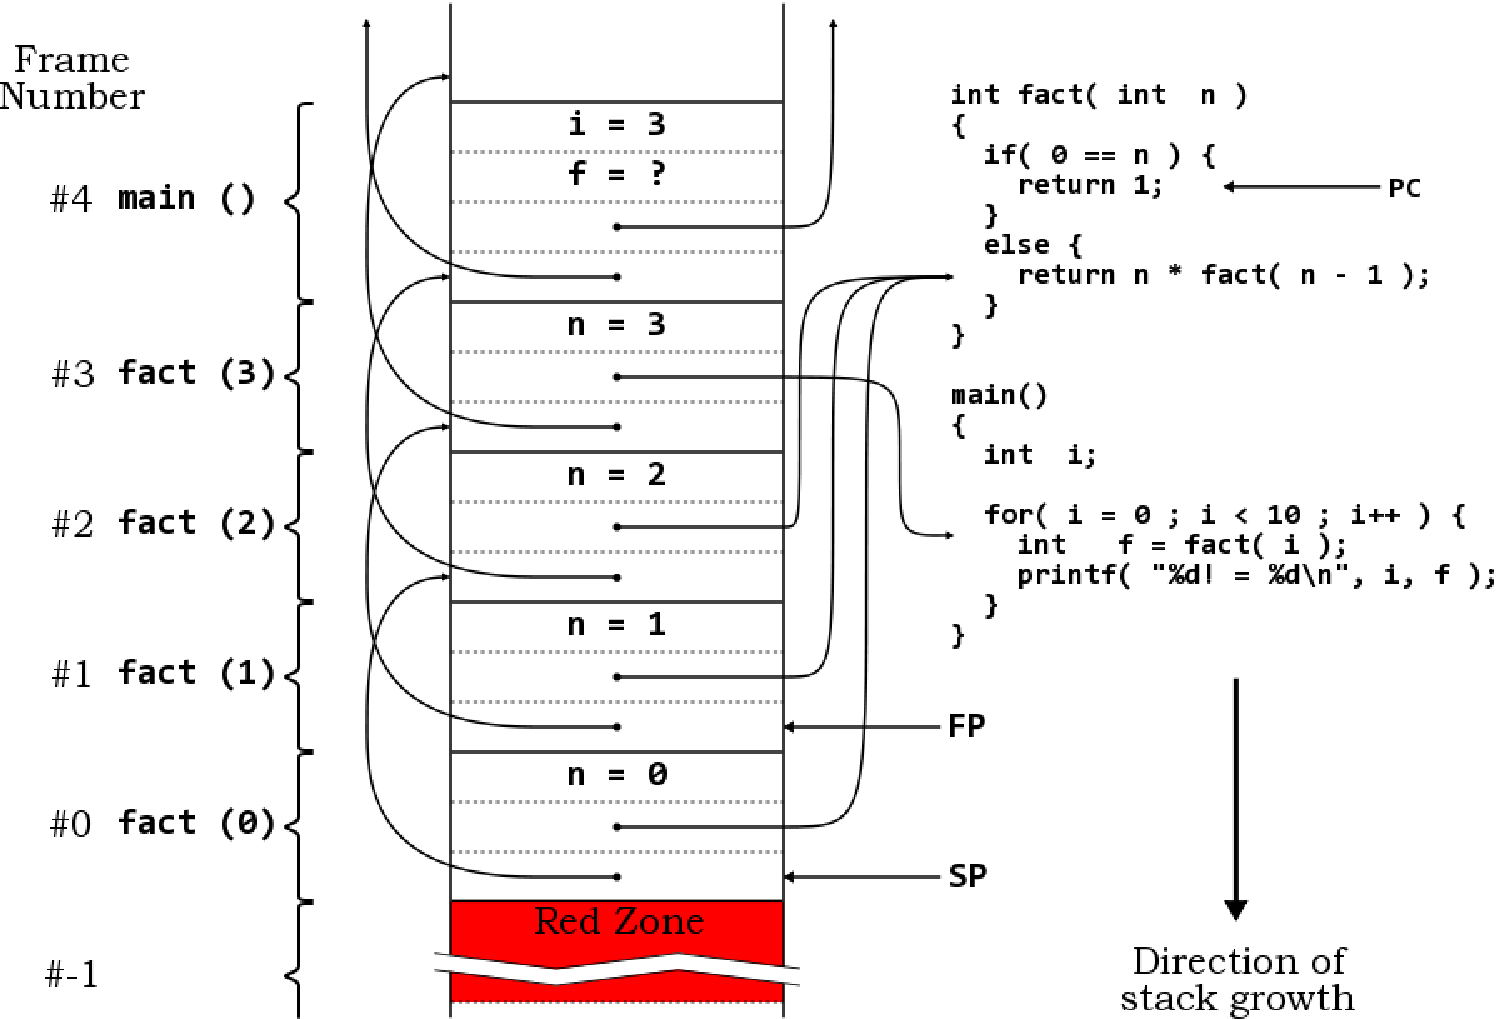
\includegraphics[width=0.9\textwidth]{figure/stack_frame}
\caption{栈和帧} \label{fig:stack_frame}
\end{center}
\end{figure}

图~\ref{fig:stack}~是一个更详细的描述栈和帧的图。
\begin{figure}
\begin{center}
% 缩放到文本宽度的90%
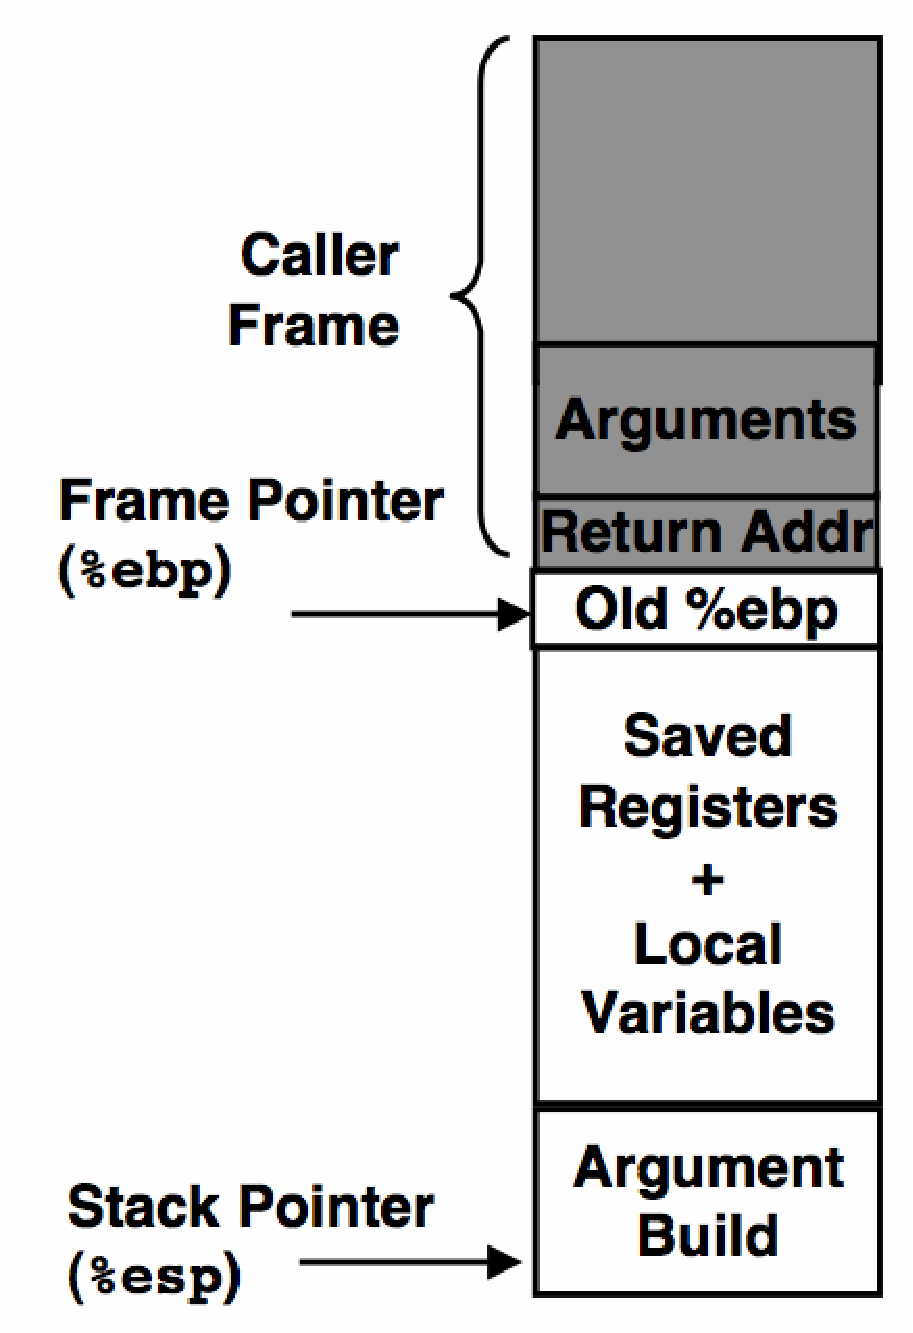
\includegraphics[scale=0.3]{figure/stack}
\caption{栈的结构} \label{fig:stack}
\end{center}
\end{figure}

调试程序很方便的一点,也是非常重要的一点就是停止在断点是可以看到断点所在的调用栈,它告诉你被调试的程序执行到了什么地方,是怎么执行到这里的。
通过对栈的检查,还能看到函数调用时使用的参数,
以及被调用到函数的局部变量等信息。
在~GDB~中,程序的调用栈看起来像这样:
\begin{lstlisting}
(gdb) bt
#0  0x00a1a7a2 in _dl_sysinfo_int80 () from /lib/ld-linux.so.2
#1  0x00c85f7c in pthread_cond_timedwait@@GLIBC_2.3.2 () from /lib/tls/libpthread.so.0
#2  0x0805f271 in ACE_OS::cond_timedwait (this=0x0, abstime=0xb7ffc2a0)
    at /home/cm/ACE_wrappers/ace/OS.i:2772
#3  0x0805f271 in ACE_Condition_Thread_Mutex::wait (this=0x0, abstime=0xb7ffc2a0)
#4  0x0805f271 in ACE_Condition_Thread_Mutex::wait (this=0x0, abstime=0xb7ffc2a0)
#5  0x0804d224 in ACE_Message_Queue<ACE_MT_SYNCH>::wait_not_empty_cond (this=0x80af8b8, mon=...,
    timeout=0xb7ffc2a0) at /home/cm/ACE_wrappers/ace/Message_Queue_T.cpp:1139
#6  0x0804d914 in ACE_Message_Queue<ACE_MT_SYNCH>::dequeue_head (this=0x80af8b8, first_item=@0xb7ffc2bc,
    timeout=0xb7ffc2a0) at /home/cm/ACE_wrappers/ace/Message_Queue_T.cpp:1296
#7  0x0804cf46 in ACE_Task<ACE_MT_SYNCH>::getq (this=0xbffff390, mb=@0xb7ffc2bc, tv=0xb7ffc2a0)
    at /home/cm/ACE_wrappers/ace/Task_T.i:21
#8  0x0804cdfb in cm::TaskManager::svc (this=0xbffff390) at foo.cpp:61
#9  0x0806bf38 in ACE_Task_Base::svc_run (args=0xbffff390) at Task.cpp:203
#10 0x08066d0a in ACE_Thread_Adapter::invoke_i (this=0x80afb38) at Thread_Adapter.cpp:148
#11 0x08066c8a in ACE_Thread_Adapter::invoke (this=0x80afb38) at Thread_Adapter.cpp:91
#12 0x00c833cc in start_thread () from /lib/tls/libpthread.so.0
#13 0x00afd1ae in clone () from /lib/tls/libc.so.6
\end{lstlisting}

检查栈主要使用下面这些命令:

\noindent
\code{backtrace [\param{full}] [\param{n}|\param{-n}]} \index{gdb!backtrace} \index{gdb!bt}

打印出出程序的调用栈。命令缩写为~\code{bt}。
可选参数~\param{full}~表示在打印栈的每一帧时同时打印出该帧上函授调用的参数及函数的局部变量。
可选参数~\param{n}~或~\param{-n}~表示要打印的调用栈的帧数。
如果是正数~\param{n}~表示从栈顶(最后调用的函数)开始计数打印~\param{n}~帧,
如果是负数~\param{-n}~表示从栈底(main函数)开始计数打印~\param{n}~帧。


\subsection{帧(frame)}
因为栈是由帧组成的,所以检查栈上的数据,其实就是和帧打交道。
每一帧包含了函数调用的参数,函数的局部变量以及正在执行的函数的地址。
当程序启动的时候,栈上只有一帧(就是~\code{main}~函数),
通常这一帧称为初始帧(\emph{initial frame})或者最外面的帧(\emph{outermost frame}),
每进行一次函数调用产生新的一帧,当函数调用返回的时候,该帧被销毁。如果函数是递归调用的,会有不停的新的帧产生,如果调用的深度太深,就会导致栈被耗尽。

在程序内部,帧使用帧的地址来标识,
通常会有一个\emph{帧寄存器}用来保存当前帧的指针。

GDB~会对每一帧给以一个编号,最里面的帧(当前正在执行的帧)的编号为~0,
调用它的函数的帧的变化为~1,以此类推\ldots
帧的编号在~GDB~调试中命令会用到。

有些编译器提供了一种优化可以把栈帧优化掉。比如~GCC~提供了优化选项
\code{-fomit-frame-pointer}可以把帧指针优化掉。
GDB~不能很好的处理这类函数调用,因此建议在编译调试版本时不要使用这个优化选项。

和帧相关的命令有下面这些:

\noindent
\code{frame \param{n}}

\paramdesc{切换到第~\param{n}~帧。命令缩写为~\code{f}。
该命令会显示切换到的帧的函数名、参数及指令地址等信息。}


\noindent
\code{up \param{n}}

\paramdesc{向上移动~\param{n}~帧。如果参数缺省:\param{n}=1。
比如当前在第~0~帧的话,\code{up}~之后就移动到第~1~帧了。}

\noindent
\code{down \param{n}}

\paramdesc{向下移动~\param{n}~帧。如果参数缺省:\param{n}=1。
比如当前在第~5~帧的话,\code{up}~之后就移动到第~4~帧了。}

\noindent
\code{info frame [\param{addr}]}

\paramdesc{打印~\param{addr}~所在帧的所有信息,
包括调用帧、参数、局部变量、寄存器等信息。
如果没有指定参数~\param{addr},默认为当前帧。}

\noindent
\code{info args}

\paramdesc{打印当前帧的函数调用的参数。}

\noindent
\code{info locals}

\paramdesc{打印当前帧的局部变量。}

\noindent
\code{info catch}

\paramdesc{打印当前帧的异常捕获句柄。}


示例:
\begin{lstlisting}
(gdb) frame 8
#8  0x0804cdfb in cm::TaskManager::svc (this=0xbffff390) at foo.cpp:61
61	                    if (this->getq(mb, &timeout) < 0) {
(gdb) info args
this = 0xbffff390
(gdb) info frame
Stack level 8, frame at 0xb7ffc320:
 eip = 0x804cdfb in cm::TaskManager::svc (foo.cpp:61); saved eip 0x806bf38
 called by frame at 0xb7ffc360, caller of frame at 0xb7ffc270
 source language c++.
 Arglist at 0xb7ffc318, args: this=0xbffff390
 Locals at 0xb7ffc318, Previous frame's sp is 0xb7ffc320
 Saved registers:
  ebx at 0xb7ffc314, ebp at 0xb7ffc318, eip at 0xb7ffc31c
(gdb) info locals
mb = 0x0
timeout = {...}
workers = {...}
...
\end{lstlisting}


\section{检查源代码}

\subsection{打印源代码}

在~GDB~中使用命令~\code{list}\index{gdb!list}(缩写为~\code{l}~)打印源码,
\code{list}~命令有下面几种格式:

\noindent
\code{list}

\paramdesc{打印当前正在执行的代码。
默认打印源代码的行数为~10~行。
如果重复执行该命令,会连续的打印出紧邻的源代码,
比如上一次~\code{list}~命令打印的源代码行号的范围为213\~222,
那么~\code{list}~命令打印的源代码行号的范围为223\~232。}

\noindent
\code{list [\param{filename}:]\param{lineno}}

\paramdesc{打印指定源文件~\param{filename}~和行号~\param{lineno}~处的代码。
如果没有指定~\param{filename},使用当前正在执行的源代码所在的源文件。}

\noindent
\code{list \param{function}}

\paramdesc{打印指定函数的源代码。}

\noindent
\code{list \param{*address}}

\paramdesc{打印地址~\param{address}~处的源代码。}

\noindent
\code{list -}

\paramdesc{向前打印源代码。
比如上一个~\code{list}~命令打印的源代码行号范围为1138\~1147,
那么~\code{list -}~命令打印的源代码行号范围为1128\~1137。}

\code{list}~命令默认打印的行数为~10~行。
如果要修改打印的行数,需要使用~\code{set listsize}~命令。

\noindent
\code{set listsize \param{count}}

\paramdesc{修改~\code{list}~命令一次打印的源代码的行数。}

\noindent
\code{show listsize}

\paramdesc{显示~\code{list}~命令一次打印的源代码的行数。}

\code{list}~的使用示例:
\begin{lstlisting}
(gdb) list
(gdb) list 1123
(gdb) list foo
\end{lstlisting}

\subsection{编辑源代码}

在调试的时候,发现错误可以立即修改源代码,然后编译之后再继续调试。
GDB~早已经实现这种功能,我们可以使用~\code{edit}~\index{gdb!edit}命令修改源代码。
编辑完成之后执行~\code{make}~命令立即编译,
然后可以在执行~\code{run}~命令重新开始调试。
在重新调试的时候,之前设置的断点依然有效。

\noindent
\code{edit [\param{filename}:]\param{lineno}}

\paramdesc{编辑指定文件~\param{filename}~和指定行号~\param{lineno}~处的源代码。
如果没有指定~\param{filename},使用当前正在执行的代码所在的源代码。}

\noindent
\code{edit \param{function}}

\paramdesc{编辑指定函数~\param{function}~所在的源文件,并定位到该函数。}

\noindent
\code{edit}

\paramdesc{如果不指定参数。编辑当前正在执行的的代码所在的源文件。}

在编辑源代码的时候~GDB~会使用环境变量~\code{EDITOR}~所指定的编辑器作为源代码编辑器。
比如如果你想使用~vim~作为源代码编辑器,需要在执行~\code{gdb}~之前先设置该环境变量。
对于~\code{bash}~的~\code{SHELL},命令为
\begin{lstlisting}
export EDITOR=vim
\end{lstlisting}
对于~\code{csh}~的~\code{SHELL},命令为
\begin{lstlisting}
setenv EDITOR vim
\end{lstlisting}
如果需要保存设置,对于~\code{bash}~的~\code{SHELL},
可以把设置写入~\code{\~/.bash\_profile}。
对于~\code{csh}~的~\code{SHELL},
可以把设置写入~\code{\~/.cshrc}。

\subsection{查找源代码}

在~GDB~中还可以通过关键字字查找源代码,
对应的命令为~\code{search}~和~\code{reverse-search}:
\index{gdb!search} \index{gdb!reverse-search}

\noindent
\code{forward-search \param{regexp}} \\
\code{search \param{regexp}}

\paramdesc{在当前源文件正向查找~\param{regexp},
参数~\param{regexp}~支持正则表达式。命令缩写为~\code{fo}。}


\noindent
\code{reverse-search \param{regexp}}

\paramdesc{在当前源文件反向查找~\param{regexp},
参数~\param{regexp}~支持正则表达式。命令缩写为~\code{rev}。}

示例:
%TODO
\begin{lstlisting}

\end{lstlisting}


\subsection{指定源代码的搜索路径}

在使用~\code{list}~命令的时候,有时候会因为编译的机器和调试的不是同一台的机器的原因,
或者调试时源代码的路径发生了改变,这可能导致~GDB~无法打印源代码。

\noindent
\code{directory \param{dirname} \ldots}

\paramdesc{设置源代码的搜索路径。命令的缩写为~\code{dir}。
针对~UNIX~平台,多个路径名之间使用冒号(:)分隔,
针对~WIN~平台,多个路径名之间使用分号(;)分隔。
使用使用变量~\code{\$cdir}~代表编译目录,
变量~\code{\$cwd}~代表当前工作目录。
}

\noindent
\code{directory}

\paramdesc{重新设置源代码的搜索路径为初始值。
比如在UNIX平台上该值的设置为~\code{\$cdir:\$cwd}。
执行该命令后会提示你确认。}


\noindent
\code{show directories}

\paramdesc{打印源代码的搜索路径。}

示例:
%TODO
\begin{lstlisting}

\end{lstlisting}


\subsection{反汇编}

在~GDB~中可以使用命令~\code{disassemble}~来进行反汇编源代码。

\noindent
\code{disassemble [\param{/m}|\param{/r}] [\param{addr}|\param{func}]}

\paramdesc{从指定的地址~\param{addr}~开始反汇编,
或者反汇编指定的函数~\param{func},
如果没有指定~\param{addr}~和~\param{func},
反汇编当前正在执行的指令。
参数~\param{/m}~指定反汇编的时候同时打印对应的源代码,
参数~\param{/r}~指定反汇编的时候同时打印对应的~16~进制的机器指令。}

示例:
%TODO
\begin{lstlisting}

\end{lstlisting}


\section{检查数据}

调试的时候免不了要打印某个变量的值,数组的值,某个内存地址值等信息。
GDB~提供了丰富的命令来打印这些信息。
GDB~还支持类型之间的强制转换,对数组的操作。

GDB~提供的检查数据的命令有~\code{print}、\code{printf}、\code{x}、\code{output}、
\code{display}~等。

\subsection{打印表达式的值 - \code{print}}

打印某个表达式最常用的命令是~\code{print},缩写为~\code{p}。

\noindent
\code{print [\param{/fmt}] \param{expr}}

\paramdesc{打印表达式~\param{expr}~的值,
可以使用使用参数~\param{fmt}~来进行强制格式转换后再打印,
默认是使用定义的数据类型来打印。
\param{fmt}~支持的格式见表~\ref{tab:print_fmt}。}

\begin{table}[!bhp]
\begin{tabularx}{400pt}{l|X}
\hline
\hline
fmt & 说明 \\
\hline
x & 把~\param{expr}~转换为整数并以~16~进制的格式打印。\\
d & 把~\param{expr}~转换为有符号整数并以~10~进制的格式打印。\\
u & 把~\param{expr}~转换为无符号整数并以~16~进制的格式打印。\\
o & 把~\param{expr}~转换为整数并以~8~进制的格式打印。\\
t & 把~\param{expr}~转换为整数并以~2~进制的格式打印。t代表的含义是two。\\
a & 把~\param{expr}~作为一个地址打印。类似命令~\code{info symbol \param{expr}}。\\
o & 把~\param{expr}~转换为char并打印,如果是不可打印字符,使用'$\backslash$nnn'的格式表示。\\
f & 把~\param{expr}~转换为浮点数并打印。\\
s & 把~\param{expr}~转换为以'$\backslash$0'结尾的字符串并打印。\\
\hline
\hline
\end{tabularx}
\caption{print支持的格式}\label{tab:print_fmt}
\end{table}

\noindent
\code{printf \param{template}, \param{expr}\ldots}

\paramdesc{使用~C~语言的风格的printf来打印表达式~\param{expr}~的值,
多个~\param{expr}~之间使用逗号分隔。}

示例
\begin{lstlisting}
p i
p/x $pc
printf
%TODO
\end{lstlisting}

\subsection{数组}

GDB~支持打印数组,
表达数组在~GDB~中的格式为~\code{\param{array}@\param{len}}。
其中~\param{array}~为数组的名称,\param{len}~为数组的长度。

比如在~C++~中这样定义一个包含3个元素的数组:
\begin{lstlisting}
int* ia = new int[3];
\end{lstlisting}
数组的内容为{111, 222, 333},
我们可以使用~\code{print *ia@3}~来打印数组的内容。
示例如下:

\begin{lstlisting}
(gdb) p ia@3
$4 = {0x87f8018, 0x87f8008, 0xbfe54e78}
(gdb) p *ia@3
$5 = {111, 222, 333}
(gdb) p ia
$6 = (int *) 0x87f8018
(gdb) p *ia
$7 = 111
\end{lstlisting}


\subsection{打印内存中的信息 - \code{x}}

要检查任意内存处的数据,可以使用命令~\code{x}(examine~的缩写)。

\noindent
\code{x\param{/nfu addr}}

\paramdesc{打印内存~\param{addr}~处的数据。
参数~\param{n},\param{f},\param{u}~是可选参数。}

\paramdesc{参数~\param{n}~指定要检查的内存长度,单位由参数~\param{u}~指定。缺省为1。}

\paramdesc{参数~\param{f}~指定打印的格式,参见表~\ref{tab:print_fmt},
另外新增一种格式~\code{i},表示打印汇编指令(instructions)。
缺省为~\code{x}。}

\paramdesc{参数~\param{u}~指定打印的单位。支持的单位见表~\ref{tab:x_param_unit}。
缺省值为~\code{w}。}

\begin{table}
\begin{tabularx}{400pt}{l|X}
\hline
\hline
u & 说明 \\
\hline
b & Bytes.  \\
h & Halfwords (two bytes).  \\
w & Words (four bytes). This is the initial default. \\
g & Giant words (eight bytes). \\
\hline
\hline
\end{tabularx}
\caption{x命令支持的打印单位}\label{tab:x_param_unit}
\end{table}

比如,\code{x/10cb 0x12345}~打印从内存地址~\code{0x12345}~开始处~10(参数\param{n})个~byte(参数\param{b})的字符(参数\param{c})。
\code{x/12xw \$sp}~打印栈指针开始处~12~个字长的~16~进制数。
\code{x/6i \$eip}~打印当前指令接下来的6条指令。使用~\code{x/i \$eip}~可以查看当前正在执行的指令。

示例:
%TODO
\begin{lstlisting}

\end{lstlisting}

\subsection{自动打印某个表达式的值 - \code{display}}

当你要频繁的监视一个表达式的值的时候
(比如在~\code{for}~循环中,打印循环的次数),
使用命令~\code{display}~可以很方便完成这种任务。
\code{display}~会在每次程序中断的时候自动进行打印。

\noindent
\code{display [\param{/fmt}] \param{expr}}

\paramdesc{当程序中断的时候自动打印表达式~\param{expr}~的值。
比如每执行一次~\code{next}~命令,~\param{expr}~的值都会被打印一次。
参数\param{/fmt}~见表~\ref{tab:print_fmt},
另外可以使用~\code{i}~来打印指令。
设置成功后返回一个编号来代表该监视的表达式,
这个编号可以用于删除和禁用该自动监视的表达式。}

\noindent
\code{display}

\paramdesc{打印所有设置了要自动监视的表达式的值。}

\noindent
\code{undisplay \param{dnums} \ldots} \\
\code{delete display \param{dnums} \ldots}

\paramdesc{删除之前使用~\code{display}~设置的要自动监视的表达式。
\param{dnums}~由~\code{display}~命令返回。}

\noindent
\code{disable display \param{dnums} \ldots}

\paramdesc{禁用之前使用~\code{display}~设置的要自动监视的表达式。
\param{dnums}~由~\code{display}~命令返回。}

\noindent
\code{enable display \param{dnums} \ldots}

\paramdesc{启用之前使用~\code{disable}~禁用的自动监视的表达式。
\param{dnums}~由~\code{display}~命令返回。}

\noindent
\code{info display}

\paramdesc{打印所有要自动监视的表达式列表。}

示例:
%TODO

\subsection{打印设置}

GDB~可以控制打印时的一些格式,典型的设置如下:

\noindent
\code{set print pretty \param{on}|\param{off}}

\paramdesc{设置打印~\code{struct/union/class}~的成员时是否分行打印,
设置为~\param{on}~开起来效果要好些,但是如果成员变量很多时就会占用很多行。
效果参见本节的示例。
缺省为~\param{off}。}

\noindent
\code{show print pretty}

\paramdesc{显示~\code{set print pretty}~的设置。}

\noindent
\code{set print object \param{on}|\param{off}}

\paramdesc{}

\noindent
\code{show print object}

\paramdesc{缺省为~\param{on}。}

\noindent
\code{set print vtble \param{on}|\param{off}}

\paramdesc{是否答应C++虚函数表。缺省为~\param{on}。}

\noindent
\code{show print vtble}

\paramdesc{}

\subsection{历史记录}

\code{print}~打印的表达式的值~GDB~都会记录下来,
GDB~在打印的时候会给该表达式指定一个编号~\param{num},
后续在其它的表达式中可以使用~\$\param{num}~来直接引用该表达式的值。

\noindent
\code{show values [\param{n}]}

\paramdesc{打印~GDB~记录的表达式值的历史。
如果指定参数~\param{n},那么最多打印~\param{n}~个历史表达式的值。}

示例:
%TODO

\subsection{内部变量}

\noindent
\code{\$\_}

\paramdesc{}


\noindent
\code{\$\_\_}

\paramdesc{}

\noindent
\code{\$\_exitcode}

\paramdesc{}

\noindent
\code{\$\_siginfo}

\paramdesc{}

\subsection{寄存器}

GDB~中可以打印的寄存器的值,寄存器使用~\$\param{regname},
\param{regname}~是寄存器的名字。
可以使用~\code{info registers}~来打印寄存器信息。

\noindent
\code{info registers}

\paramdesc{打印当前帧除了浮点数和向量寄存器的其它所有寄存器的名字和值。}

\noindent
\code{info all-registers}

\paramdesc{打印当前帧所有寄存器(包括浮点数和向量寄存器)的名字和值。}

示例:
%TODO

\begin{lstlisting}
info registers
p $eax
x/i $eip
\end{lstlisting}

\subsection{如何产生core}

在调试的时候如果想保存正在调试的程序的当前状态以后再来继续分析,
可以通过产生~core~文件来达到此目的。
关于~core~的调试,参考第~\ref{ch:coredump}~章(第~\pageref{ch:coredump}~页)。

\noindent
\code{generate-core-file [\param{file}]}\\
\code{gcore [\param{file}]}

\paramdesc{生成当前正在调试的文件~core~文件,
参数~\param{file}~用于指定~core~文件名,
如果没有指定,默认为~core.\param{pid},
\param{pid}是正在调试的进程的进程号。}

示例:
\begin{lstlisting}
(gdb) gcore
Saved corefile core.6945
(gdb) gcore foo.dump
Saved corefile foo.dump
\end{lstlisting}


\subsection{在内存中查找}

在~GDB~中可以使用~\code{find}~命令在内存中进行搜索。

\noindent
\code{find [\param{/sn}] \param{start\_addr, +len}, \param{val1} [, \param{val2} \ldots]} \\
\code{find [\param{/sn}] \param{start\_addr, end\_addr}, \param{val1} [, \param{val2} \ldots]}

\paramdesc{在指定的内存中查找指定的序列~\param{val1},\param{val2}\ldots
指定的内存要求是连续的,
可以指定开始地址(\param{start\_addr})和长度(\param{len}),
或者指定开始地址(\param{start\_addr})和结束地址(\param{end\_addr})。
\param{s}~和~\param{n}~是可选参数。}

% TODO:

\section{修改执行路径}
在调试时可以通过下面的方法更改程序的执行路径:
\begin{itemize}
\item 修改变量的值
(参见第~\ref{sec:modvar}~节,第~\pageref{sec:modvar}~页);

\item 让函数提前返回并指定想要的返回值
(参见第~\ref{sec:cmd_return}~节,第~\pageref{sec:cmd_return}~页);

\item 给程序发送信号
(参见第~\ref{sec:sendsignal}~节,第~\pageref{sec:sendsignal}~页);

\item 调用指定的函数
(参见第~\ref{sec:cmd_return}~节,第~\pageref{sec:cmd_return}~页);

\end{itemize}

GDB~甚至还能修改你正在调试的二进制文件,俗称patch
(参见第~\ref{sec:makepatch}~节,第~\pageref{sec:makepatch}~页)。

\subsection{修改变量的值}
\label{sec:modvar}

GDB~中可以使用~\code{print}~命令和~\code{set}~来对变量进行赋值。
\code{print}~赋值后之后会打印出新的值,
而~\code{set}~不会打印新的值。
如果不知道要赋值的变量的类型,可以使用~\code{ptype}~来查看。

\noindent
\code{set \param{name} = \param{value}}

\paramdesc{给变量~\param{name}~赋值~\param{value}。}

\noindent
\code{set \{\param{type}\}\param{addr} = \param{value}}

\paramdesc{把内存地址为~\param{addr}存储的数据强制类型转换成~\param{type},
并且赋值为~\param{value}。
示例:\code{set \{int\}0x8aaa01c = 1234}。
}

\noindent
\code{ptype \param{var}}

\paramdesc{打印变量~\param{var}~的类型定义。
比如~\param{var}~是一个class的实例,它会打印该~class~的定义。}

示例:
\begin{lstlisting}
% TODO
p i = 1
set x = 2
set {int}0xddfd = 3
\end{lstlisting}

\subsection{直接跳转}

在调试过程中,可以使用~~命令直接跳转到指定的地址出继续执行。

\noindent
\code{jump \param{lineno}}\\
\code{jump \param{addr}}

\paramdesc{跳转到指定的行号~\param{lineno}~或指定的地址~\param{addr}。
一般预先在掉转的目标地址设置好一次性断点,
在跳转之后就会立即停在这个断点上。
\code{jump}~不会改变当前帧、栈、内存及寄存器的值\footnote{除了指令寄存器PC。},
所以跳转最好在本函数内进行。}

\paramdesc{在某些平台上,可以通过修改寄存器~PC~的值来达到同样的效果。}

\subsection{发送信号}
\label{sec:sendsignal}

在调试的时候,可以向被调试的程序发送信号,使用~\code{signal}~命令。

\noindent
\code{signal \shparam{signo}}

\paramdesc{向被调试的程序发送信号~\param{signo}。
\param{signo}~可以是数字或信号名,
比如~\code{signal 1}~和~\code{signal SIGHUP}~的效果是一样的。}

\paramdesc{如果~\param{signo}~为~0,表示继续执行程序而不处理信号。
在因为信号被中断的情况下,
如果想使程序忽略这个信号继续执行就应该使用“\code{signal 0}”,
而不是~\code{continue},因为~\code{continue}~不会忽略信号。}

\subsection{提前返回}
\label{sec:cmd_return}

在调试的过程可以使用~\code{return}~命令来从当前函数提前返回。

\noindent
\code{return [\param{expression}]}

\paramdesc{不执行当前函数剩下的代码而直接返回。
可选参数~\param{expression}~可以用来指定函数的返回值。
如果你想执行完当前函数然后再返回,应该使用~\code{finish}~命令(第~\pageref{sec:cmd_finish}~页)。}

\subsection{调用函数}

在调试的过程中,可以使用~\code{print}~或~\code{call}~命令调用其它的函数并执行。

\noindent
\code{print \param{func}}\\
\code{call \param{func}}

\paramdesc{执行函数~\param{func}。}

如果函数~\param{func}~执行过程中产生信号,
可以通过~\code{set unwindonsignal}~来控制其行为。
在调用~\code{call}~之前应该先调用~\code{set unwindonsignal}。

\noindent
\code{set unwindonsignal \param{on}|\param{off}}

\paramdesc{如果设置为~\param{on},在~\code{call}~命令执行完之后,
把堆栈恢复到之前的状态。
如果设置为~\param{off},如果在执行~\param{func}~的过程中产生信号,
程序会中断在~\param{func}~中。
缺省为~\param{off}。
}

\code{show unwindonsignal}

\noindent{显示~\code{set unwindonsignal}~的设置。}

\subsection{制作patch}
\label{sec:makepatch}

缺省情况下,GDB~以只读的方式打开被调试的文件和~core~文件。
如果你需要~patch~它们,需要在~GDB~启动的时候指定~\shparam{-write}~参数或者使用~\gdbcmd{set write}~命令。

\noindent
\gdbcmd{set write \gdbcmdparam{on}|\gdbcmdparam{off}}

\paramdesc{设置当前正在调试的二进制文件和~core~文件是否可写。缺省为~\gdbcmdparam{off}。}

\noindent
\gdbcmd{show write}

\paramdesc{显示当前正在调试的可执行文件和~core~文件是否可写。}

示例:
\begin{lstlisting}
$ gdb ./a.out
(gdb) show write
Writing into executable and core files is off.
(gdb) set write on
(gdb) show write
Writing into executable and core files is on.
\end{lstlisting}


\section{GDB的文本界面(TUI)}
\label{sec:tui}
GDB~支持curses的文本窗口模式,称之为TUI - Text User Interface。
TUI能显示如下四个窗口:
GDB在单独的窗口中显示源文件、汇编代码、寄存器信息及GDB的命令输入/输出。

启动TUI的方式是使用~'gdbtui'~或~'gdb -tui'。

\section{自定义GDB命令}

GDB~支持自定义命令,就是说你可以把~GDB~的几个命令组合成新的自定义命令,
而且在自定义的命令中能使用~\gdbcmd{if}~进行条件判断,
使用~\gdbcmd{while}~进行循环等。
自定义命令使用~\gdbcmd{define}~来完成。

\begin{lstlisting}
define cmdname
 ...
 ...
end

document cmdname
  There is help of cmdname.
end
\end{lstlisting}

自定义命令最多可以有~10~个参数,
它们是~\gdbcmdparam{\$arg0}\ldots\gdbcmdparam{\$arg9}。
在命令体中可以使用\gdbcmdparam{\$argc}~来代表传递的参数个数。
\gdbcmd{document}~是可选的,用来定义该自定义命令的帮助信息,
如果定义的话,在~\gdbcmd{help} \gdbcmdparam{cmdname}~的时候会显示该帮助信息。

示例一:需要一个参数的自定义命令:
\begin{lstlisting}
define get_chunk
  if $argc == 1
    set $addr = $arg0
    print (($addr - malloc_start)/4096)*140 + heap_start
  else
    echo Usage: get_chunk addr
  end
end
\end{lstlisting}

在用户自定义的命令中使用~\gdbcmd{if}~的语法如下:
\begin{lstlisting}
if cond
  ...
else
  ...
end
\end{lstlisting}

在用户自定义的命令中使用~\gdbcmd{while}~的语法如下:
\begin{lstlisting}
while cond
  ...
end
\end{lstlisting}

\subsection{定义GDB命令Hook}

在~GDB~中可以定义~GDB~命令的~Hook,即对于~GDB~的命令~\gdbcmd{cmdname},
如果存在自定义的命令~\gdbcmd{foo-cmdname},
那么在执行~\gdbcmd{cmdname}~的时候,会先执行~\gdbcmd{foo-cmdname}。

%TODO: example

\section{GDB初始化文件}

在~GDB~每次启动的时候,都会尝试读取它的初始化文件\$HOME/.gdbinit
并执行。如果想在.gdbinit中执行其它的文件,可以使用source命令。

\noindent
\gdbcmd{source \gdbcmdparam{file}}
\index{gdb!source}

\paramdesc{执行~\gdbcmdparam{file}~中的命令。}


\section{逆向调试(Reverse Debug)}
\index{gdb!逆向调试}

在程序调试时候,你是否有过因为随手的\code{n}就执行一条语句,
之后你才意识意识到你并不想执行\code{n}命令。
一般来说,为了再次遇到这个条件,这就意味这你要重头开始再来调试一次了,
这个时候要是有后悔药就好了,可以回退到之前的状态再来一次,
这样就极大可以加快调试的速度。

\section{GDB的文本界面(TUI)}
GDB~支持curses的文本窗口模式,称之为TUI-Text User Interface。
TUI能显示如下四个窗口:
GDB在单独的窗口中显示源文件、汇编代码、寄存器信息及GDB的命令输入/输出。

启动TUI的方式是使用~'gdbtui'~或~'gdb -tui'。
如果是~GDB~的~shell~下,可以使用组合键~\shcmd{Ctrl-x a}(按住Ctrl同时按x,然后释放Ctrl和x,再按a)来切换到TUI模式。

\subsection{TUI中的组合键}

在~GDB~中支持的组合键如下:

\noindent
\gdbcmd{Ctrl-x a}

\paramdesc{进入或退出TUI模式。}


\noindent
\gdbcmd{Ctrl-x 1}

\paramdesc{只显示~1~个窗口:源代码或汇编窗口。
如果~TUI~没有启动,它会自动启动~TUI。}

\noindent
\gdbcmd{Ctrl-x 2}

\paramdesc{至少打开~2~个窗口。
如果~TUI~没有启动,它会自动启动~TUI。}

\noindent
\gdbcmd{Ctrl-x o}

\paramdesc{改变当前活动的窗口。}

\noindent
\gdbcmd{Ctrl-L}

\paramdesc{刷新当前屏幕。
在调试的时候,如果被调试的平、程序有向屏幕输出的话,
可能会把屏幕弄的很难看,这个时候~\gdbcmd{Ctrl-L}~就派上用场了。}

\subsection{TUI涉及的命令}

\noindent
\gdbcmd{layout next}

\paramdesc{切换到下一个窗口布局模式。
重复该命令,GDB会自动在几种窗口布局中进行切换。
你可以选择你想要的布局模式然后停下来。}

\noindent
\gdbcmd{layout prev}

\paramdesc{切换到上一个窗口布局模式。}

\noindent
\gdbcmd{layout src}

\paramdesc{只显示源代码窗口。}

\noindent
\gdbcmd{layout asm}

\paramdesc{只显示汇编代码窗口。}

\noindent
\gdbcmd{layout split}

\paramdesc{同时显示源代码与汇编代码窗口。}

\section{GDB高级用法}

\subsection{GDB初始化文件}

\subsection{自定义GDB命令}


\section{逆向调试(Reverse Debug)}
\index{gdb!逆向调试}

在程序调试时候,你是否有过因为随手的\code{n}就执行一条语句,
之后你才意识意识到你并不想执行\code{n}命令。
一般来说,为了再次遇到这个条件,这就意味这你要重头开始再来调试一次了,
这个时候要是有后悔药就好了,可以回退到之前的状态再来一次,
这样就极大可以加快调试的速度。
在不确定程序bug的时候,使用逆向调试也是很有帮助的,
可以在可能产生错误的地方反复调试,最终找到bug的根源。

在GDB 7.0的版本开始支持\emph{逆向调试}。
\emph{逆向调试}当前仅在有限的平台上支持,
\code{i386}和\code{amd64}是支持\emph{逆向调试}的。

\emph{逆向调试}中用到的命令:

\noindent
\code{reverse-continue}(缩写为'rc')

Continue program being debugged but run it in reverse

\noindent
\code{reverse-finish}

Execute backward until just before the selected stack frame is called

\noindent
\code{reverse-next} ('rn')

Step program backward, proceeding through subroutine calls.

\noindent
\code{reverse-nexti} ('rni')

Step backward one instruction, but proceed through called subroutines.


\noindent
\code{reverse-step} ('rs')

Step program backward until it reaches the beginning of a previous source line

\noindent
\code{reverse-stepi}

Step backward exactly one instruction

\noindent
\code{set exec-direction [\param{forward}|\param{reverse}]}

Set direction of execution.

All subsequent execution commands (continue, step, until etc.) will run the program being debugged in the selected direction.

Breakpoints and watchpoints will work in reverse -- allowing you for instance to proceed directly to the previous point at which a variable was modified.


https://sourceware.org/gdb/wiki/ReverseDebug



\section{使用GDB查看STL容器}
\index{gdb!查看STL容器}

如果是用~GDB~的\emph{print}命令来打印~STL~容器(如~vector,stack,set~等),
得到的结果是很难读。

\subsection{GDB 7.0}
GDB7.0能通过Python的pretty-printers\index{gdb!pretty-printers}支持更友好的打印STL容器的信息。

设置步骤如下:

1. 获取~Python libstdc++~的printers:
\begin{lstlisting}[language={sh}]
mkdir -p ~/.gdb/gdb_printers
cd ~/.gdb/gdb_printers
svn co svn://gcc.gnu.org/svn/gcc/trunk/libstdc++-v3/python
\end{lstlisting}

2. 修改\emph{\$HOME/.gdbinit},添加如下几行:
\begin{lstlisting}
python
import sys
sys.path.insert(0, '/home/maude/gdb_printers/python')
from libstdcxx.v6.printers import register_libstdcxx_printers
register_libstdcxx_printers (None)
end
\end{lstlisting}

\subsection{GDB 6.x}
现实是现在Linux发行版中很少有使用~GDB 7.0~的。但是通过~GDB~的自定义命令,
可以很方便的查看STL容器的内容。Dan Marinescu已经写了这样一个GDB的宏包,
当前版本是1.0.3,文件名是stl-view-1.0.3.gdb。

使用方法:
把stl-view-1.0.3.gdb放在\emph{\$HOME/.gdb/}下。
在\emph{\$HOME/.gdbinit}中加入如下一行:
\begin{lstlisting}
source ~/.gdb/stl-view-1.0.3.gdb
\end{lstlisting}

然后可以使用下表的命令来打印STL容器的内容
\index{gdb!pvector} \index{gdb!plist} \index{gdb!pmap} \index{gdb!pset}
\index{gdb!pdequeue} \index{gdb!pstack}
\begin{table}[!bhp]
\begin{tabular}{l|l}
\hline
\hline
容器类型 & GDB命令      \\
\hline
std::vector<T>          &       pvector stl\_variable    \\
std::list<T>	        &       plist stl\_variable T    \\
std::map<T,T>	        &       pmap stl\_variable       \\
std::multimap<T,T>      &       pmap stl\_variable       \\
std::set<T>	        &       pset stl\_variable T     \\
std::multiset<T>        &       pset stl\_variable       \\
std::deque<T>	        &       pdequeue stl\_variable   \\
std::stack<T>	        &       pstack stl\_variable     \\
std::queue<T>	        &       pqueue stl\_variable     \\
std::priority\_queue<T>	&       ppqueue stl\_variable    \\
std::bitset<n>td>	&       pbitset stl\_variable    \\
std::string	        &       pstring stl\_variable    \\
std::widestring	        &       pwstring stl\_variable   \\
\hline
\hline
\end{tabular}
\caption{打印STL容器的GDB命令列表}
\end{table}

\subsection{使用示例}
std::vector<int> iv;
在gdb中使用pvector来打印出iv的内容:\\
(gdb) pvector iv;

%TODO: 范例

更多的信息参考:
https://sourceware.org/gdb/wiki/STLSupport\cite{gdb-stl-support}

\section{GDB的图像界面DDD}
\index{DDD}

\section{F.A.Q}

\begin{enumerate}
\item \textbf{Q}:在~GDB~的输出有很多行时会提示
“Type <return> to continue, or q <return> to quit“,
如何取消这个限制,让~GDB~一次性完成输出?

\textbf{A}:使用\code{set height 0}或者\code{set pagination off}。

\item \textbf{Q}:在~\code{print}~命令中类型强制转换:
\code{p *(cm::Foo*)0x85cf008},
提示“A syntax error in expression, near `)0x85cf008'”,
如何解决?

\textbf{A}:这是因为”\code{::}“的原因,
需要使用单引号把要要转换的类型引起来,
像这样:\code{p *('cm::Foo'*)0x85cf008}~就可以了。

\item \textbf{Q}:如何调试C++的异常?

\textbf{A}:\emph{方法一}:可以使用~GDB~的~\code{catch throw}~在catch上设置\emph{catchpoint}
(参见第~\ref{sec:gdb_catchpoint}~节,第~\pageref{sec:gdb_catchpoint}~页)。

\emph{方法二}:如果程序是使用~GCC~编译器编译的话,
可以在函数~\code{\_Unwind\_RaiseException}~上设置断点。
效果和\emph{方法一}类似。

\emph{方法三}:如果你已经知道要\code{throw}的名称,
而且这个异常是你自己定义的异常,
那么你还可以在你的异常类的构造函数上设置断点。

\item \textbf{Q}:我的~GDB~版本是~6.3,我想在上面调试~C++~异常,
可是~\code{catch throw}~返回错误:
“Function "\_\_cxa\_throw" not defined”,我该怎么办?

\textbf{A}:升级到GDB 7.0。

\item \textbf{Q}:使用~GDB~检查~core~文件时候提示:
“BFD: Warning: foo-15591.core is truncated: expected core file size >= 616845312, found: 314601472.”,这是怎么回事?
\begin{lstlisting}
(gdb) bt
#0  0x082fb2d8 in std::list<xmlnode*, std::allocator<xmlnode*> >::empty (this=Cannot access memory at address 0xb6b70160)
    at /usr/lib/gcc/i386-redhat-linux/3.4.6/../../../../include/c++/3.4.6/bits/stl_list.h:671
Cannot access memory at address 0xb6b7015c
\end{lstlisting}

\textbf{A}:core~文件被截断了。可能的原因有:

\emph{原因一}:产生~core~的时候磁盘没有空间了?

\emph{原因二}:系统设置了~core~文件的大小限制,
对于是~\code{bash}~的~\code{SHELL},使用命令“\code{ulimit -c}”检查,
如果设置了限制,使用命令“\code{ulimit -c unlimited}”取消限制。
如果~\code{csh}的~\code{SHELL}~对应的命令为~\code{limit}。


\item \textbf{Q}:

\textbf{A}:

\end{enumerate}



\section{总结}

关于GDB的更多信息参见GDB在线手册\cite{gdb-man}。

关于GDB的书籍有:

Debugging with GDB: The GNU Source-Level Debugger\cite{debugging-with-gdb}。
在网上能找到这本书的电子版。本章的大部分内容来自该书。

GDB Pocket Reference\cite{gdb-pocket-ref}。

GDB~的在线文档:
https://sourceware.org/gdb/download/onlinedocs/


\chapter{内存问题}
\section{简介}
C/C++语言因为没有垃圾回收机制,需要应用程序自身对内存进行管理,
这就可能导致内存管理的混乱。下面列举一些常见的内存相关的问题:

\begin{itemize}
\item 访问已经被释放的内存空间;
\item 释放已经被释放的内存;
\item 重叠的内存操纵,比如memcpy时源地址和目的地址有重叠的情况
\end{itemize}

\section{缓冲区溢出}

\emph{缓冲区溢出}\index{缓冲区溢出}(Buffer overflow)~现在被越来越多的人知道了,
大家都知道它给操作系统及网络安全带来了严重的安全隐患,
在CERT(http://www.cert.org)中报告的问题中\emph{缓冲区溢出}一直是占有最大的比例。

作为一个程序员,如何编写安全的代码,避免缓冲区溢出,
提高程序的健壮性是本节的目的。

\subsection{缓冲区溢出的原理}
\emph{缓冲区溢出}(Buffer overflow)是由于C语言缺乏类型安全引起的,

\subsection{缓冲区溢出的预防}

对C语言来说,在对字符串进行操作时,遵循如下规则:

\begin{itemize}
\item 使用strncpy代替strcpy
\item 使用strncat代替strcat
\item 避免使用puts,scanf
\end{itemize}

\subsubsection{编写安全的代码}

\subsubsection{使用工具预防缓冲区溢出}

TODO: https://www.cert.org/secure-coding/


\section{匿名对象的生命周期}

如下一段代码有一个内存相关的bug:

\begin{lstlisting}[language={C++},numbers=left]
std::ostringstream oss;
...
...
printf("oss: %s\n", s.str().c_str());
\end{lstlisting}

\emph{c\_str()} 产生了一个临时临时变量,在 \emph{printf()} 要使用的时候可能已经从栈上消失了,
程序运行的结果就是可能打印出来的是乱码,因为 \emph{c\_str()} 返回的内存地址已经不是有效的内存地址了。

Book: Thinking in C++


\section{调试内存问题的工具}

TODO


% -*- coding: utf-8 -*-

\chapter{信号}


\section{僵尸(Zombie)进程}

\subsection{僵尸进程产生的原因}

在~fork~产生子进程后,当子进程先于父进程退出时,
虽然内核会释放它的内存和其它相关的资源,
但为了要父进程获取子进程的退出状态,
内核会保留这个已退出进程的相关信息,
典型的信息会包括子进程的退出状态,
子进程的累积的CPU占有时间。
这些信息会在父进程调用wait或waitpid的时候返回给父进程。
在子进程退出后,但父进程还没有调用wait或waitpid的这段时间里,
这个已经退出的子进程成为\emph{僵尸(Zombie)进程}\index{Zombie}\index{僵尸进程}。

进程退出时,它的父进程会收到一个SIGCHLD信号。
一般情况下,这个信号的句柄通常执行wait系统调用,
这样处于僵死状态的进程会被删除。
如果父进程没有这么做,子进程会一直处于僵尸状态。
实际上,僵尸进程不会对系统有大的危害,顶多就是它占用一个pid,
看起来''碍眼''。

\subsection{如何杀掉僵尸进程}

僵尸进程的状态在Linux/HP-UX中被标识了Z。在top命令的S列如果有进程显示为Z,则表示该进程是僵尸进程。

在Linux中,僵尸进程会被标识成~[defunct],可以用下面的命令查找系统中的僵尸进程:
\begin{lstlisting}
ps -ef | grep defunct
\end{lstlisting}

你会发现使用kill命令(即使你使用-KILL参数也是没有用)
是不能杀死这种进程的\footnote{僵尸怎么可能被杀死呢?}。
原因是它已经退出了,什么也没有了,自然无法收到任何信号。

既然知道僵尸进程产生原因,杀掉僵尸\footnote{杀掉这种说法并不准确,
因为僵尸进程本身已经结束了。这里的“杀掉”只是指把僵尸进程从进程表里删除掉。}
的思路就是让它的父进程执行\code{wait}或\code{waitpid}调用来处理~SIGCHLD~信号。
有两种方法可以做到这一点:

\begin{enumerate}
\item 一种方法是改变僵尸进程的父进程。
用kill命令杀死它的父进程,这样init变成它的新的父进程,
而init会定时地执行wait系统调用。

\item 另一种方式是使用调试器,在父进程中执行\code{wait}系统调用。
调用~GDB~执行如下命令: 
\begin{lstlisting}
gdb parent-progname parent-pid
(gdb) set unwindonsignal on 
(gdb) call wait(pid-of-zombie-process) 
\end{lstlisting}

gdb会在父进程中调用wait,从而达到我们的目的。
注意,unwindonsignal\index{gdb!unwindonsignal}要被set为on, 
它告诉gdb把堆栈恢复到调用\code{wait}之前的状态。
要不然父进程会crash。 

\end{enumerate}

\subsection{如何编程避免僵尸进程的产生}
在程序中避免僵尸进程除了显式调用\code{wait}或\code{waitpid}外,
也可以使用下面的代码忽略~SIGCHLD~信号来避免僵尸进程,
使用这种方法不好的一个方面就是父进程不再能够获得子进程的退出状态了。

\begin{lstlisting}
   struct sigaction sa; 
   sa.sa_handler = SIG_IGN; 
   sa.sa_flags = SA_NOCLDWAIT; 
   sigemptyset (&sa.sa_mask); 
   sigaction (SIGCHLD, &sa, NULL); 
\end{lstlisting}

参考exit(2)手册页。 


%# -*- coding: utf-8 -*-

\chapter{多线程的调试}
\label{ch_mt} \index{多线程的调试}

\section{简介}

\section{线程安全问题}
\index{线程安全}

\section{饥饿}
线程无限期的等待资源而不能获得。
比如低优先级线程等待的资源总是被高优先级线程获取。

\section{死锁问题} \index{死锁}

\subsection{导致死锁的原因}
导致死锁至少有两个锁在互相争用。
Mutual exclusion
Only one thread at a time can use a resource.

Hold and wait
Thread holding at least one resource is waiting to acquire additional resources held by other threads

No preemption
Resources are released only voluntarily by the thread holding the resource, after thread is finished with it

Circular wait
There exists a set {T1, \ldots, Tn} of waiting threads
  T1 is waiting for a resource that is held by T2
  T2 is waiting for a resource that is held by T3
  ...
  Tn is waiting for a resource that is held by T1

\subsection{死锁检测} \index{死锁检测}

\subsection{死锁检测算法}
Only one of each type of resource $\rightarrow$ look for loops

更一般的死锁检测算法
Let [X] represent an m-ary vector of non-negative 
integers (quantities of resources of each type):
    用[X]代表包含m个元素的数组,m为每种类型的资源数目:
    [FreeResources]代表当前可用的资源;
    [RequestX]代表来自线程X的请求;
    [AllocX]代表线程X获得的资源。

    检查一个任务是否能最终完成的算法如下:
        
See if tasks can eventually terminate on their own

\begin{lstlisting}
[Avail] = [FreeResources] 
Add all nodes to UNFINISHED 	
do {
  done = true
  Foreach node in UNFINISHED {	
    if ([Requestnode] <= [Avail]) {
      remove node from UNFINISHED
      [Avail] = [Avail] + [Allocnode]
      done = false
    }
   }
} until(done)				
\end{lstlisting}
如果UNFINISHED非空,那么就有死锁产生了。


应用程序本身是无法检查到死锁的。

\begin{table}
\caption{分析程序挂起状态的脚本}
\begin{lstlisting}[language={sh}]
#!/bin/sh

if [ $# -ne 1 ] ; then
  echo "Usage: $0 <pid>"
  exit 1
fi

pid=$1

\end{lstlisting}
\end{table}

\subsection{如何避免死锁}
死锁的避免\index{死锁避免}需要从设计上进行

当检测到死锁时,需要进行如下操作:

Terminate thread, force it to give up resources
\begin{itemize}
\item[-]结束线程,强迫该线程放弃资源。

In Bridge example, Godzilla picks up a car, hurls it into the river.  Deadlock solved!
Shoot a dining lawyer
But, not always possible – killing a thread holding a mutex leaves world inconsistent

Preempt resources without killing off thread 
\item[-]抢占资源而不需要结束线程。

Take away resources from thread temporarily
Doesn’t always fit with semantics of computation

Roll back actions of deadlocked threads 
\item[-]回滚会导致死锁的线程。
在数据库的操作中,为了保证事务的原子性,这种方式使用的比较多。
    Hit the rewind button on TiVo, pretend last few minutes never happened
For bridge example, make one car roll backwards (may require others behind him)
Common technique in databases (transactions)
Of course, if you restart in exactly the same way, may reenter deadlock once again

\end{itemize}


\section{Monitor}
Monitor~\index{Monitor}是使用一把锁和一个或多个条件变量来保护在并发中的共享数据的一种方式。
Monitor~代表的逻辑是:
\begin{itemize}
\item[-] 等待如果需要的话;
\item[-] 当条件满足的时候唤醒等待在该条件上的线程继续执行。
\end{itemize}

在\emph{生产者/消费者}模型中,为了同步\emph{生产者}和\emph{消费者}线程,
Monitor~被广泛的使用。 
Monitor主要依靠\emph{条件变量}来实现,
一个\emph{条件变量}需要和一个\emph{锁}关联起来。
Monitor~是一个很容易产生错误的模式,这里举例说明通常使用Monitor的方式。

消费者线程:
\begin{lstlisting}
...
pthread_mutex_lock(&lock);
while (condition is false) {          // check and/or update 
  pthread_cond_wait(&condvar, &lock); // state variables
}                                     // wait if necessary
pthread_mutex_unlock(&lock);
...
\end{lstlisting}
\code{pthread\_cond\_wait()}\index{pthread\_cond\_wait}的语义要求原子的完成如下两个操作:
\begin{enumerate}
\item 释放之前已经获得的锁\param{lock};
\item 调用线程进入睡眠状态,直到其它的线程调用\code{pthread\_cond\_signal()}来唤醒自己。
\end{enumerate}
在\code{pthread\_cond\_wait()}返回的时候,它会自动获取在睡眠之前释放的锁\param{lock}。

\emph{说明}:
\begin{enumerate}
\item 在调用\code{pthread\_cond\_wait()}之前一定要先获得\emph{条件变量}使用的\emph{锁}\param{lock}。
\item 在\code{pthread\_cond\_wait()}返回之后我们通常要再次测试条件是否满足,
因为可能存在假的唤醒操作\footnote{我们的程序的应该尽量避免这种假的唤醒,但是有时候还是很难避免的。}。
这就是为什么要使用while而不是if的原因了。这里也是容易产生错误的地方。
\end{enumerate}

生产者线程:
\begin{lstlisting}
...
pthread_mutex_lock(&lock);

// check and/or update state variables
if (condition is true)
  pthread_cond_signal(&condvar);
pthread_mutex_unlock(&lock);

...
\end{lstlisting}

\emph{说明}:
\begin{enumerate}
\item 在条件变成真的时候,调用\code{pthread\_cond\_signal()}\index{pthread\_cond\_signal}来唤醒等待在该条件上的线程。
\item 这段代码可能导致潜在的\emph{锁竞争}\index{锁竞争}。
设想在比较极端的情况下,在\code{pthread\_cond\_signal()}被调用后,
等待在该条件上线程立即被唤醒了,并被调度开始立即执行,
这个时候它会因为不能获取\emph{锁}\param{lock}而立刻停止。
解决这种锁争用的方法之一是把\code{pthread\_cond\_signal()}的调用放在\code{pthread\_mutex\_unlock()}之后。
修改后的代码看起来想这样:
\begin{lstlisting}
...
pthread_mutex_lock(&lock);

// check and/or update state variables
pthread_mutex_unlock(&lock);

if (condition is true)
  pthread_cond_signal(&condvar);
...
\end{lstlisting}
\end{enumerate}





\section{如何调试多线程的程序}

\subsection{使用valgrind来调试多线程程序}
valgrind~\index{valgrind}提供了对多线程进行分析的工具,能发现多线程中的问题。
版本3.5.0的valgrind提供如下工具进行多线程的调试。

\subsection{使用Intel的线程检查器来调试多线程程序} 
\index{Intel线程检查器}
Intel~提供线程检查器(Intel\textregistered Thread Checker)了多线程的调试工具,
可以在~x86~的~Linux~平台下使用。它能检查应用程序的竞争与死锁等问题。
并准确的在源代码层找到错误的位置以及出错的调用栈。
使用方法


\section{总结}

更多关于Intel线程检查的信息参考Intel官方网站\cite{intel-thread-checker}



%# -*- coding: utf-8 -*-

\chapter{Core dump的调试}
\label{ch:coredump}

\section{产生coredump的原因}

core dump\index{coredump}分为主动产生和被动产生的,
比如主动调用\code{abort()}命令就会主动产生coredump。

另一种产生~core dump~的原因是程序收到了一下信号\index{信号}会产生core dump。
会产生~core dump~的信号\footnote{关于信号的更多信息参见man 7 signal。}见表~\ref{sec:tab_core_signals}~所示。

\begin{table}[!hbp]
\caption{产生core dump的信号列表} \label{sec:tab_core_signals}
\begin{tabular}{l|c|l}
\hline
信号名 & 信号值 & 信号描述 \\
\hline
SIGQUIT &    3	&	Quit from keyboard \\
SIGILL  &    4	&	Illegal Instruction \\
SIGABRT &    6	&	Abort signal from abort(3) \\
SIGFPE  &    8	&	Floating point exception \\
SIGSEGV &    11	&	Invalid memory reference \\
SIGBUS  &    10,7,10 &	Bus error (bad memory access) \\
SIGSYS  &    12,-,12 &	Bad argument to routine (SVID) \\
SIGTRAP &    5	&	Trace/breakpoint trap \\
SIGXCPU &    24,24,30 & CPU time limit exceeded (4.2 BSD) \\
SIGXFSZ &    25,25,31 & File size limit exceeded (4.2 BSD) \\
SIGIOT  &    6	&	IOT trap. A synonym for SIGABRT \\
\hline
\end{tabular}
\end{table}

某些信号的\emph{信号值}这一列对应有三个值,因为信号是平台相关的,
在不同的平台上有不同的值。第一个是alpha和sparc平台定义的该信号的值,
第二个是i386,ppc和sh平台定义的该信号的值,
第三个值是mips平台定义该信号的值。
如果是-表示该平台没有实现该信号。

\section{Linux下core dump的配置}
\subsection{控制是否产生core dump}
在Linux下是否产生从core dump文件以及对产生的core dump的大小限制是可配置的,
在Bash/sh/ksh下可以使用ulimit\footnote{csh的命令是limit。}\index{ulimit}命令来查看该设置:\\
\begin{lstlisting}
$ ulimit -c
1000000
\end{lstlisting}
如果输出是0表示不产生core dump文件,
这个时候为了获得core dump就需要修改这个参数,
把它改成一个正数或者unlimited表示对core dump的文件大小没有限制。

\begin{lstlisting}
$ ulimit -c unlimited
$ ulimit -c
unlimited
\end{lstlisting}

\subsection{定制core dump的文件名}

有的Linux默认的core dump的文件名就是core,有的是core.<pid>,
一般core dump的产生于程序的当前运行目录。

对于~Linux 2.5~以上的版本,我们可以通过配置Linux的内核参数
\emph{kernel.core\_pattern}\index{kern.core\_pattern}
来指定core dump的产生位置及文件名,这个文件名是一个模板,
在文件名中可以使用~\%~开头的修饰符来,
在实际产生core dump文件的时候会根据这个修饰符来做相应的替换。
可用的修饰符见表~\ref{sec:tab_core_pattern}~所示。

\begin{table}
\begin{tabular}{r|l}
\hline
通配符 & 含义   \\
\hline
\%\%  &   A single \% character    \\
\%p  &   PID of dumped process   \\
\%u  &   real UID of dumped process  \\
\%g  &   real GID of dumped process  \\
\%s  &   number of signal causing dump   \\
\%t  &   time of dump (secs since 0:00h, 1 Jan 1970) \\
\%h  &   hostname (same as the 'nodename' returned by uname(2))  \\
\%e  &   executable filename \\
\hline
\end{tabular}
\caption{kern.core\_pattern可用的修饰符}\label{sec:tab_core_pattern}
\end{table}

比如如果我们指定core dump文件名的名字模板为
\begin{lstlisting}
/var/crash/%e-%p-%s.core
\end{lstlisting}

如果我们有一个名为test\_fmr,
进程号为24214的的进程因为SIGSEGV信号而异常退出了,
它会在~/var/crash~下生成一个如下一个core dump文件:
\begin{lstlisting}
/var/crash/test_fmr-24214-11.core
\end{lstlisting}

\emph{kern.core\_pattern}~也可以通过proc文件系统来进行配置,
它在/proc文件系统中的位置为:
\begin{lstlisting}
/proc/sys/kernel/core_pattern
\end{lstlisting}

如果是~Linux 2.4~的版本,由于没有内核参数\emph{kernel.core\_pattern},
它对core dump的文件名的控制功能就没有自如了,还好它也有一个内核参数
\emph{kernel.core\_uses\_pid}
\footnote{这个参数在新版本的内核是被遗弃的,不再建议使用。}
\index{kern.core\_uses\_pid},
可以用来控制core生成时是否包含进程的pid的。
它的值可以是0或其它值,
如果是0则产生的core dump的文件简单的命名为core,
否则的话产生的core dump文件格式为core.PID。
\emph{kernel.core\_uses\_pid}在/proc文件系统中的位置为:
\begin{lstlisting}
/proc/sys/kernel/core_uses_pid
\end{lstlisting}

可以通过sysctl、/etc/sysctl.conf或/proc文件系统来修改这两个参数,
只有修改~/etc/sysctl.conf~才会永久生效。

示例:
\begin{lstlisting}
# sysctl -w kernel.core_pattern=/var/crash/%e-%p-%s.core
\end{lstlisting}

修改~/etc/sysctl.conf~后需要执行如下命令来从新读入~/etc/sysctl.conf:
\begin{lstlisting}
# sysctl -p
\end{lstlisting}

我们可以借助valgrind(参见\ref{valgrind},第\pageref{valgrind}页)、
yamd(参见\ref{yamd},第\pageref{yamd}页)等工具来帮助我们发现程序的内存错误。

\subsection{捕获会导致core dump的信号}

下面的代码能捕获并处理SIGSEGV信号:

\lstinputlisting[language={C++},numbers=left]{code/segv_handler.cpp}
\begin{figure}
\caption{捕获会导致core dump的信号的代码}
\end{figure}

链接的时候需要指定~\code{-rdynamic -ldl}~选项,这样才能获得栈上的信息。

\subsection{定位出错的源代码行}
调用栈会给出每一帧的地址,我们需要知道这个地址来获得源代码的对应的
行号来定位出现问题的代码。可以使用~GDB~的~\code{list}~命令来定位,如下所示:
\begin{lstlisting}
$ gdb foo
(gdb) l *0x804904a
0x804904a is in Foo::run() (test_signal.cpp:181).
\end{lstlisting}

另外一种方式就是通过addr2line\index{addr2line}来获得:
%\begin{lstlisting}[language={sh}]
\begin{lstlisting}
$ addr2line -e foo 0x804904a
/home/cm/sandbox/test_signal.cpp:181
\end{lstlisting}

\subsection{C++名字重整}
\index{c++filt}

可以通过这篇文章获取更多的在程序在收到SIGSEGV信号时获取调用栈的信息:\\
Obtaining a stack trace in C upon SIGSEGV\cite{obtain-sigsegv-stack}

\subsection{C++类的内存布局}

针对~GCC~编译后的C++程序,如果一个类存在虚函数,
那么它的内存布局的第一个成员时虚表指针,然后才是其它的成员函数。

参考下面的代码演示了类~\code{Bar}~的内存布局。

\begin{lstlisting}
#include <stdlib.h>

class Foo
{
    public:
        Foo()
        {
            x = 0x12345678;
            y = 0x98765432;
            p = (void*)0x3c3c3c3c;
        }

        virtual void run() { }

        virtual ~Foo() { }

    private:
        int x;
        int y;
        void* p;
};

class Bar : public Foo
{
    public:
        Bar() : b(911) {}

        virtual void run() { }

    private:
        int b;
};

int main()
{
    Bar* f = new Bar;
    abort();
}
\end{lstlisting}

通过~GDB~我们可以清楚的看到~\code{Bar}~的内存布局,
它的第一个成员变量即为虚表指针。

\begin{lstlisting}
$ gdb ./a.out
Program received signal SIGABRT, Aborted.
0x0012d422 in __kernel_vsyscall ()
(gdb) f 3
#3  0x0804860f in main () at memlayout.cpp:37
37          abort();
(gdb) p f
$1 = (Bar *) 0x804b008
(gdb) p *f
$2 = (Bar) {
  <Foo> = {
    _vptr.Foo = 0x8048808,
    x = 305419896,
    y = -1737075662,
    p = 0x3c3c3c3c
  },
  members of Bar:
  b = 911
}
(gdb) x/8x f
0x804b008:      0x08048808      0x12345678      0x98765432      0x3c3c3c3c
0x804b018:      0x0000038f      0x00020fe9      0x00000000      0x00000000
\end{lstlisting}

\section{使用GDB分析core dump文件}

\begin{table}
\begin{tabularx}{400pt}{l|X}
\hline
GDB命令 & 说明 \\
\hline
bt                  &   查看core的调用栈    \\
bt full		        &   查看得完整调用栈信息,包含每一帧的参数值及局部变量的值等 \\
thread apply all bt &   查看所有线程的调用栈 \\
frame $n$           &   切换到调用栈的第~$n$~帧 \\
info threads	    &   查看当前的函数的线程的信息(包括有多少个线程及每个线程的栈顶) \\
info frame 	        &   查看当前帧的信息 \\
info local          &   查看当前函数局部变量的值 \\
info reg		    &   查看寄存器的值 \\
\hline
\end{tabularx}
\caption{GDB调试core dump的常用命令}
\end{table}


\section{调试其它机器上产生的core dump文件}

core dump文件是程序在异常退出时内存的映像。

为了减少core dump文件的大小,core dump文件只保存了可写的节的内存映像,
而没有包含程序的可执行代码(不可变的)。

调试其它机器上产生的core dump文件不仅需要其它导致core dump的可执行程序,
而且还需要它依赖的动态库,否则的话使用bt命令可能看到不是正确的结果。

\subsection{示例}

使用~GDB~的~\code{info shared}\index{info shared}
来获取可执行程序依赖的动态库列表。
然后把这些动态库打包。

在产生core dump的机器上执行把这些动态库打包:

\begin{lstlisting}
$ gdb ust ust-3124.core
(gdb) info shared
From       To         Syms Read Shared Object Library
0x4001e44c 0x40026e80 Yes       /rlib/libpthread.so.0
0x4004d9a0 0x4006adac Yes       /usr/lib/libstdc++-libc6.2-2.so.3
0x4007faa0 0x400966b4 Yes       /rlib/libm.so.6
0x400ba590 0x40197bb4 Yes       /rlib/libc.so.6
0x40001fe0 0x40013808 Yes       /lib/ld-linux.so.2
0x401fa454 0x40200310 Yes       /lib/libnss_files.so.2
0x40203010 0x40204c50 Yes       /lib/libnss_dns.so.2
0x40208c48 0x40212480 Yes       /lib/libresolv.so.2
(gdb) quit
$ cd /
$ tar czf ust_solibs_orig.tar.gz        \
    /rlib/libpthread.so.0               \
    /usr/lib/libstdc++-libc6.2-2.so.3   \
    /rlib/libm.so.6             \
    /rlib/libc.so.6             \
    /lib/ld-linux.so.2          \
    /lib/libnss_files.so.2      \
    /lib/libnss_dns.so.2        \
    /lib/libresolv.so.2
\end{lstlisting}

然后把产生的core dump的可执行文件、
core dump文件以及依赖的动态库拷贝到目标机器上。
使用gdb的~\code{set solib-absolute-prefix}\index{solibs-absolute-prefix}
来设置可执行程序的加载的动态库的绝对路径。


\begin{lstlisting}
$ mkdir /home/cm/ust_solibs_orig
$ cd /home/cm/ust_solibs_orig
$ tar zxf ust_solibs_orig.tar.gz
$ gdb ust
(gdb) set solib-absolute-prefix /home/cm/ust_solibs_orig
(gdb) core ust-3124.core
(gdb) bt
(gdb) bt full
\end{lstlisting}

\section{无法获得调用栈的core dump文件分析}

对于某些情况下的core dump文件,使用\code{bt}命令无法获得完整的调用栈。
这个时候需要借助于反汇编的帮助。使用 \\
\begin{lstlisting}
x/i \$eip \index{eip}
\end{lstlisting}
来查看当前的正在执行的指令,一般来说这个指令会有非法的地址访问。
示例:

使用info来查看当前的寄存器信息:\\
\begin{lstlisting}
info reg
\end{lstlisting}

结合当前的寄存器信息和当前的指令可以看出导致core的原因。

\begin{lstlisting}
Program terminated with signal 11, Segmentation fault.
Cannot access memory at address 0xb7f07000
#0  0x0826db92 in UcpfIdbAttachment::IsOmaNniAttachment (this=Cannot access memory at address 0xb6b04150) at idb/UcpfIdbAttachment.h:605
in idb/UcpfIdbAttachment.h
(gdb) bt
#0  0x0826db92 in UcpfIdbAttachment::IsOmaNniAttachment (this=Cannot access memory at address 0xb6b04150)
    at idb/UcpfIdbAttachment.h:605
Cannot access memory at address 0xb6b04148
(gdb) x/i $eip
0x826db92 <_ZNK17UcpfIdbAttachment18IsOmaNniAttachmentEv+6>:
    mov    0x10b(%eax),%al
(gdb) info reg
eax            0x0          0
ecx            0x89         137
edx            0xb250d218   -1303326184
ebx            0x1caff4     1880052
esp            0xb6b04148   0xb6b04148
ebp            0xb6b04148   0xb6b04148
esi            0x0          0
edi            0xb6b04400   -1229962240
eip            0x826db92    0x826db92
eflags         0x10292      66194
cs             0x73         115
ss             0x7b         123
ds             0xc02e007b   -1070727045
es             0x7b         123
fs             0x0          0
gs             0x33         51
\end{lstlisting}

\begin{lstlisting}
$ objdump -S foo > foo.asm
\end{lstlisting}

\begin{lstlisting}
00000000 <_ZNK17UcpfIdbAttachment18IsOmaNniAttachmentEv>:
   0:   55                      push   %ebp
   1:   89 e5                   mov    %esp,%ebp
   3:   8b 45 08                mov    0x8(%ebp),%eax
   6:   8a 80 0b 01 00 00       mov    0x10b(%eax),%al
\end{lstlisting}


\section{总结}

对于如何定制Linux下产生的core dump的文件名的更多信息请参考~Linux~的~\code{core}的手册页。


%# -*- coding: utf-8 -*-

\chapter{程序性能剖析}

\label{profile} \index{性能剖析}



\chapter{Linux内核调试}

\section{Linux内核调试基础}

\section{Oops}
\index{Oops}
Oops是内核编程中比较容易遇到的问题,为了跟多的了解Oops来便于调试,我对Oops提供的信息进行一个总结,以及如何调试Oops。


一个完整的Oops:

\begin{lstlisting}
BUG: unable to handle kernel paging request at 00316b01
IP: [<c05dd045>] netif_receive_skb+0x335/0x377
*pde = 00000000
Thread overran stack, or stack corrupted
Oops: 0000 [#1] SMP
last sysfs file: /sys/block/hda/size
Modules linked in: mymod ipv6 autofs4 nls_utf8 cifs lockd sunrpc dm_multipath 
scsi_dh video output sbs sbshc battery lp sg snd_ens1371 gameport ide_cd_mod 
snd_rawmidi cdrom snd_ac97_codec ac97_bus snd_seq_dummy snd_seq_oss 
snd_seq_midi_event snd_seq snd_seq_device snd_pcm_oss snd_mixer_oss 
parport_pc ac floppy serio_raw snd_pcm button parport rtc_cmos rtc_core 
rtc_lib snd_timer snd pcnet32 mii soundcore snd_page_alloc i2c_piix4 i2c_core 
pcspkr dm_snapshot dm_zero dm_mirror dm_region_hash dm_log dm_mod ata_piix 
libata mptspi mptscsih mptbase scsi_transport_spi sd_mod scsi_mod ext3 jbd 
uhci_hcd ohci_hcd ehci_hcd [last unloaded: mymod]

Pid: 0, comm: swapper Not tainted (2.6.30.9 #1) VMware Virtual Platform
EIP: 0060:[<c05dd045>] EFLAGS: 00010206 CPU: 0
EIP is at netif_receive_skb+0x335/0x377
EAX: 00316ae1 EBX: deb7d600 ECX: 00316ae1 EDX: e2f357c0
ESI: 00000008 EDI: de9a4800 EBP: c9403f40 ESP: c9403f10
 DS: 007b ES: 007b FS: 00d8 GS: 0000 SS: 0068
Process swapper (pid: 0, ti=c9403000 task=c0737320 task.ti=c0779000)
Stack:
 00316ae1 c07777a0 e2f787c0 00000000 00000001 00000008 00000010 deb7d600
 c9403f40 deb7d600 00000000 df5acc58 c9403fb0 e0e61db0 00000000 00000010
 de9a4bb8 de9a4b40 de9a4800 00002000 00000001 00000000 1ea2c822 deb7d600
Call Trace:
 [<e0e61db0>] ? pcnet32_poll+0x347/0x66a [pcnet32]
 [<c041f984>] ? run_rebalance_domains+0x13d/0x3ed
 [<c05df364>] ? net_rx_action+0x6a/0xf4
 [<c0429e2a>] ? __do_softirq+0x94/0x138
 [<c0429d96>] ? __do_softirq+0x0/0x138
 <IRQ> <0> [<c0429d94>] ? irq_exit+0x29/0x2b
 [<c040423b>] ? do_IRQ+0x6d/0x83
 [<c0402e89>] ? common_interrupt+0x29/0x30
 [<c040828a>] ? default_idle+0x5b/0x92
 [<c0401a92>] ? cpu_idle+0x3a/0x4e
 [<c063d84b>] ? rest_init+0x53/0x55
 [<c077f7df>] ? start_kernel+0x293/0x298
 [<c077f06a>] ? i386_start_kernel+0x6a/0x6f

d0 89 45 d8 8b 55 d0 8b 42 20 83 e8 20 89 45 d0 8b 4d d0 <8b> 41 20 0f 18 00 
90 89 c8 83 c0 20 3b 45 d4 75 a4 83 7d d8 00

EIP: [<c05dd045>] netif_receive_skb+0x335/0x377 SS:ESP 0068:c9403f10
CR2: 0000000000316b01
---[ end trace 0330855ac41edfb5 ]---
Kernel panic - not syncing: Fatal exception in interrupt
Pid: 0, comm: swapper Tainted: G      D    2.6.30.9 #1
Call Trace:
 [<c0425ff3>] panic+0x3f/0xdf
 [<c0405644>] oops_end+0x8c/0x9b
 [<c041673a>] no_context+0x10c/0x116
 [<c04168c7>] __bad_area_nosemaphore+0xe0/0xe8
 [<c0416933>] bad_area_nosemaphore+0xd/0x10
 [<c0416aa7>] do_page_fault+0xde/0x1e3
 [<c04169c9>] ? do_page_fault+0x0/0x1e3
 [<c064f38d>] error_code+0x6d/0x74
 [<c061007b>] ? tcp_v4_rcv+0x55b/0x600
 [<c04169c9>] ? do_page_fault+0x0/0x1e3
 [<c05dd045>] ? netif_receive_skb+0x335/0x377
 [<e0e61db0>] pcnet32_poll+0x347/0x66a [pcnet32]
 [<c041f984>] ? run_rebalance_domains+0x13d/0x3ed
 [<c05df364>] net_rx_action+0x6a/0xf4
 [<c0429e2a>] __do_softirq+0x94/0x138
 [<c0429d96>] ? __do_softirq+0x0/0x138
 <IRQ>  [<c0429d94>] ? irq_exit+0x29/0x2b
 [<c040423b>] ? do_IRQ+0x6d/0x83
 [<c0402e89>] ? common_interrupt+0x29/0x30
 [<c040828a>] ? default_idle+0x5b/0x92
 [<c0401a92>] ? cpu_idle+0x3a/0x4e
 [<c063d84b>] ? rest_init+0x53/0x55
 [<c077f7df>] ? start_kernel+0x293/0x298
 [<c077f06a>] ? i386_start_kernel+0x6a/0x6f
\end{lstlisting}

 

 

解析Oops的具体含义:

\begin{lstlisting}
BUG: unable to handle kernel paging request at 00316b01
IP: [<c05dd045>] netif_receive_skb+0x335/0x377
*pde = 00000000
Thread overran stack, or stack corrupted
Oops: 0000 [#1] SMP
last sysfs file: /sys/block/hda/size
Modules linked in: mymod ipv6 autofs4 nls_utf8 cifs lockd sunrpc dm_multipath 
scsi_dh video output sbs sbshc battery lp sg snd_ens1371 gameport ide_cd_mod 
snd_rawmidi cdrom snd_ac97_codec ac97_bus snd_seq_dummy snd_seq_oss 
snd_seq_midi_event snd_seq snd_seq_device snd_pcm_oss snd_mixer_oss 
parport_pc ac floppy serio_raw snd_pcm button parport rtc_cmos rtc_core 
rtc_lib snd_timer snd pcnet32 mii soundcore snd_page_alloc i2c_piix4 i2c_core 
pcspkr dm_snapshot dm_zero dm_mirror dm_region_hash dm_log dm_mod ata_piix 
libata mptspi mptscsih mptbase scsi_transport_spi sd_mod scsi_mod ext3 jbd 
uhci_hcd ohci_hcd ehci_hcd [last unloaded: mymod]
\end{lstlisting}

上面这段这个是载入的模块信息

\begin{lstlisting}
Pid: 0, comm: swapper Not tainted (2.6.30.9 #1) VMware Virtual Platform
EIP: 0060:[<c05dd045>] EFLAGS: 00010206 CPU: 0
EIP is at netif_receive_skb+0x335/0x377
\end{lstlisting}

EIP这行指明发生Oops的具体位置,我们可以通过这个来找到出现Oops的源代码的具体行。

具体方法如下:

通过使用objdump -S反汇编netif\_receice\_skb所在的目标文件,然后找到偏移量为0x355的行,
看看这行是有什么代码汇编来的,再结合寄存器的值就能分析这个Oops的原因了。

 

\begin{lstlisting}
EAX: 00316ae1 EBX: deb7d600 ECX: 00316ae1 EDX: e2f357c0
ESI: 00000008 EDI: de9a4800 EBP: c9403f40 ESP: c9403f10
 DS: 007b ES: 007b FS: 00d8 GS: 0000 SS: 0068
Process swapper (pid: 0, ti=c9403000 task=c0737320 task.ti=c0779000)
Stack:
 00316ae1 c07777a0 e2f787c0 00000000 00000001 00000008 00000010 deb7d600
 c9403f40 deb7d600 00000000 df5acc58 c9403fb0 e0e61db0 00000000 00000010
 de9a4bb8 de9a4b40 de9a4800 00002000 00000001 00000000 1ea2c822 deb7d600
\end{lstlisting}

上面这段是寄存器和栈的信息。

 

\begin{lstlisting}
Call Trace:
 [<e0e61db0>] ? pcnet32_poll+0x347/0x66a [pcnet32]
 [<c041f984>] ? run_rebalance_domains+0x13d/0x3ed
 [<c05df364>] ? net_rx_action+0x6a/0xf4
 [<c0429e2a>] ? __do_softirq+0x94/0x138
 [<c0429d96>] ? __do_softirq+0x0/0x138
 <IRQ> <0> [<c0429d94>] ? irq_exit+0x29/0x2b
 [<c040423b>] ? do_IRQ+0x6d/0x83
 [<c0402e89>] ? common_interrupt+0x29/0x30
 [<c040828a>] ? default_idle+0x5b/0x92
 [<c0401a92>] ? cpu_idle+0x3a/0x4e
 [<c063d84b>] ? rest_init+0x53/0x55
 [<c077f7df>] ? start_kernel+0x293/0x298
 [<c077f06a>] ? i386_start_kernel+0x6a/0x6f
\end{lstlisting}

发生Oops的内核栈信息。

 

\begin{lstlisting}
Code: 74 14 f0 ff 83 a8 00 00 00 8b 4d d8 89 d8 8b 53 14 57 ff 51 08 58 8b 45 
d0 89 45 d8 8b 55 d0 8b 42 20 83 e8 20 89 45 d0 8b 4d d0 <8b> 41 20 0f 18 00 
90 89 c8 83 c0 20 3b 45 d4 75 a4 83 7d d8 00
EIP: [<c05dd045>] netif_receive_skb+0x335/0x377 SS:ESP 0068:c9403f10
CR2: 0000000000316b01
---[ end trace 0330855ac41edfb5 ]---
Kernel panic - not syncing: Fatal exception in interrupt
Pid: 0, comm: swapper Tainted: G      D    2.6.30.9 #1
\end{lstlisting}

如果kernel报告Tainted,说明kernel被损坏了,在"Trainted:"后面最多会有10个字符的提示信息来表示具体的信息。每一位上使用一个字母来表示,如下:

\begin{table}[!hbp]
\caption{Trainted Kernel标志位含义}
\begin{tabularx}{400pt}{r|X}
\hline
第几位 & 含义 \\
\hline
1 & 'G': 所有的模块都是GPL的License。如果有模块缺少MODULE\_LICENSE()或者声明是Proprietary的,则为'P'。\\
2 & 'F': 如果有模块是使用 insmod -f 强制载入的。否则为空。   \\
3 & 'S': 如果Oops发生在SMP的CPU上,但这个型号的CPU还没有被认为是SMP安全的。\\
4 & 'R': 如果有模块是使用 rmmod -f 强制卸载的。否则为空。    \\
5 & 'M': 有CPU报告了Machine Check Exception,否则为空。      \\
6 & 'B': 如果有page-release函数发现一个错误的page或未知的page标志。  \\
7 & 'U': 来自用户空间的程序设置的这个标志位。                \\
8 & 'D': 内核刚刚死掉,比如Oops或者是bug。                   \\
9 & 'A': ACPI表被覆盖。                                      \\
10 & 'W': 之前kernel已经产生过警告。                         \\
\hline
\end{tabularx}
\end{table}

Tainted字符串主要的目的是告诉调试器这个kernel已经不是一个干净的kernel了。如果一个模块在加载了之后又卸载了,Tainted仍然会保持。


\begin{lstlisting}
Call Trace:
 [<c0425ff3>] panic+0x3f/0xdf
 [<c0405644>] oops_end+0x8c/0x9b
 [<c041673a>] no_context+0x10c/0x116
 [<c04168c7>] __bad_area_nosemaphore+0xe0/0xe8
 [<c0416933>] bad_area_nosemaphore+0xd/0x10
 [<c0416aa7>] do_page_fault+0xde/0x1e3
 [<c04169c9>] ? do_page_fault+0x0/0x1e3
 [<c064f38d>] error_code+0x6d/0x74
 [<c061007b>] ? tcp_v4_rcv+0x55b/0x600
 [<c04169c9>] ? do_page_fault+0x0/0x1e3
 [<c05dd045>] ? netif_receive_skb+0x335/0x377
 [<e0e61db0>] pcnet32_poll+0x347/0x66a [pcnet32]
 [<c041f984>] ? run_rebalance_domains+0x13d/0x3ed
 [<c05df364>] net_rx_action+0x6a/0xf4
 [<c0429e2a>] __do_softirq+0x94/0x138
 [<c0429d96>] ? __do_softirq+0x0/0x138
 <IRQ>  [<c0429d94>] ? irq_exit+0x29/0x2b
 [<c040423b>] ? do_IRQ+0x6d/0x83
 [<c0402e89>] ? common_interrupt+0x29/0x30
 [<c040828a>] ? default_idle+0x5b/0x92
 [<c0401a92>] ? cpu_idle+0x3a/0x4e
 [<c063d84b>] ? rest_init+0x53/0x55
 [<c077f7df>] ? start_kernel+0x293/0x298
 [<c077f06a>] ? i386_start_kernel+0x6a/0x6f
\end{lstlisting}
 

 

最后发现一篇调试Oops的专题:

paper on debugging kernel oops or hang <http://mail.nl.linux.org/kernelnewbies/2003-08/msg00347.html> 虽然是针对2.4的,但还是值得一读。


\subsection{使用VMware捕获Linux的串口输出来调试内核的Oops}
Linux的Kernel在产生Oops后会默认情况下把Oops的相关信息打印在控制台上,只有通过控制台才能看到Oops的信息,而且因为受到控制台行数限制,不能完整的看到Oops的信息,这样对调试Oops很麻烦,一种方法使用虚拟机,把串口输出指定到文件,然后再的Linux的控制台消息重定向到串口,这样可以很方便的捕获串口输出,方便调试Oops。

第一步,在VMware中设置串口输出:

Settings -> Hardware -> Add... 添加一个新的串口设备,指定使用文件输出。

第二步,在Linux中对串口进行重定向。修改 /etc/grub.conf 的kernel 行,在行尾加入如下参数:

\begin{lstlisting}
console=ttyS0,115200 console=tty0
\end{lstlisting}

重启,然后测试一下产生一个Oops,看看串口文件,如下,已经有完整的Oops的信息了:

\begin{lstlisting}
Call Trace:
0:0:0:0: [sda] Assuming drive cache: write through
sd 0:0:0:0: [sda] Assuming drive cache: write through
BUG: unable to handle kernel paging request at 00316b01
IP: [<c05dd045>] netif_receive_skb+0x335/0x377
*pde = 00000000
Thread overran stack, or stack corrupted
Oops: 0000 [#1] SMP
last sysfs file: /sys/block/hda/size
Modules linked in: mymod ipv6 autofs4 nls_utf8 cifs lockd sunrpc 
dm_multipath scsi_dh video output sbs sbshc battery lp sg snd_ens1371 
gameport ide_cd_mod snd_rawmidi cdrom snd_ac97_codec ac97_bus 
snd_seq_dummy snd_seq_oss snd_seq_midi_event snd_seq snd_seq_device 
snd_pcm_oss snd_mixer_oss parport_pc ac floppy serio_raw snd_pcm 
button parport rtc_cmos rtc_core rtc_lib snd_timer snd pcnet32 mii 
soundcore snd_page_alloc i2c_piix4 i2c_core pcspkr dm_snapshot dm_zero
dm_mirror dm_region_hash dm_log dm_mod ata_piix libata mptspi mptscsih
mptbase scsi_transport_spi sd_mod scsi_mod ext3 jbd uhci_hcd ohci_hcd 
ehci_hcd [last unloaded: mymod]

Pid: 0, comm: swapper Not tainted (2.6.30.9 #1) VMware Virtual Platform
EIP: 0060:[<c05dd045>] EFLAGS: 00010206 CPU: 0
EIP is at netif_receive_skb+0x335/0x377
EAX: 00316ae1 EBX: deb7d600 ECX: 00316ae1 EDX: e2f357c0
ESI: 00000008 EDI: de9a4800 EBP: c9403f40 ESP: c9403f10
 DS: 007b ES: 007b FS: 00d8 GS: 0000 SS: 0068
Process swapper (pid: 0, ti=c9403000 task=c0737320 task.ti=c0779000)
Stack:
 00316ae1 c07777a0 e2f787c0 00000000 00000001 00000008 00000010 deb7d600
 c9403f40 deb7d600 00000000 df5acc58 c9403fb0 e0e61db0 00000000 00000010
 de9a4bb8 de9a4b40 de9a4800 00002000 00000001 00000000 1ea2c822 deb7d600
Call Trace:
 [<e0e61db0>] ? pcnet32_poll+0x347/0x66a [pcnet32]
 [<c041f984>] ? run_rebalance_domains+0x13d/0x3ed
 [<c05df364>] ? net_rx_action+0x6a/0xf4
 [<c0429e2a>] ? __do_softirq+0x94/0x138
 [<c0429d96>] ? __do_softirq+0x0/0x138
 <IRQ> <0> [<c0429d94>] ? irq_exit+0x29/0x2b
 [<c040423b>] ? do_IRQ+0x6d/0x83
 [<c0402e89>] ? common_interrupt+0x29/0x30
 [<c040828a>] ? default_idle+0x5b/0x92
 [<c0401a92>] ? cpu_idle+0x3a/0x4e
 [<c063d84b>] ? rest_init+0x53/0x55
 [<c077f7df>] ? start_kernel+0x293/0x298
 [<c077f06a>] ? i386_start_kernel+0x6a/0x6f
Code: 74 14 f0 ff 83 a8 00 00 00 8b 4d d8 89 d8 8b 53 14 57 ff 51 08 58 
8b 45 d0 89 45 d8 8b 55 d0 8b 42 20 83 e8 20 89 45 d0 8b 4d d0 <8b> 41 
20 0f 18 00 90 89 c8 83 c0 20 3b 45 d4 75 a4 83 7d d8 00
EIP: [<c05dd045>] netif_receive_skb+0x335/0x377 SS:ESP 0068:c9403f10
CR2: 0000000000316b01
---[ end trace 0330855ac41edfb5 ]---
Kernel panic - not syncing: Fatal exception in interrupt
Pid: 0, comm: swapper Tainted: G      D    2.6.30.9 #1
Call Trace:
 [<c0425ff3>] panic+0x3f/0xdf
 [<c0405644>] oops_end+0x8c/0x9b
 [<c041673a>] no_context+0x10c/0x116
 [<c04168c7>] __bad_area_nosemaphore+0xe0/0xe8
 [<c0416933>] bad_area_nosemaphore+0xd/0x10
 [<c0416aa7>] do_page_fault+0xde/0x1e3
 [<c04169c9>] ? do_page_fault+0x0/0x1e3
 [<c064f38d>] error_code+0x6d/0x74
 [<c061007b>] ? tcp_v4_rcv+0x55b/0x600
 [<c04169c9>] ? do_page_fault+0x0/0x1e3
 [<c05dd045>] ? netif_receive_skb+0x335/0x377
 [<e0e61db0>] pcnet32_poll+0x347/0x66a [pcnet32]
 [<c041f984>] ? run_rebalance_domains+0x13d/0x3ed
 [<c05df364>] net_rx_action+0x6a/0xf4
 [<c0429e2a>] __do_softirq+0x94/0x138
 [<c0429d96>] ? __do_softirq+0x0/0x138
 <IRQ>  [<c0429d94>] ? irq_exit+0x29/0x2b
 [<c040423b>] ? do_IRQ+0x6d/0x83
 [<c0402e89>] ? common_interrupt+0x29/0x30
 [<c040828a>] ? default_idle+0x5b/0x92
 [<c0401a92>] ? cpu_idle+0x3a/0x4e
 [<c063d84b>] ? rest_init+0x53/0x55
 [<c077f7df>] ? start_kernel+0x293/0x298
 [<c077f06a>] ? i386_start_kernel+0x6a/0x6f
\end{lstlisting}


\subsection{Kdump}
\index{kdump}

Kdump是一种调试Linux内核的方法,用于在Linux内核出现Oops之后自动dump内核映像到指定位置的机制,编译我们的事后调试。

Kdump is a new kernel crash dumping mechanism and is very reliable. The crash dump is
captured from the context of a freshly booted kernel and not from the context of the crashed
kernel. Kdump uses kexec to boot into a second kernel whenever the system crashes. This
second kernel, often called a capture kernel, boots with very little memory and captures the
dump image.

1. Install kexec-tools

\begin{lstlisting}
yum install kexec-tools
\end{lstlisting}

2. write kdump config file /etc/kdump.conf with following content.

\begin{lstlisting}
path /var/crash
core_collector makedumpfile -d 31 -c
\end{lstlisting}

3. change /etc/grub.conf append crashkernel=128M@16M to the end of kernel line. example:

\begin{lstlisting}
default=0
timeout=5
splashimage=(hd0,0)/grub/splash.xpm.gz
hiddenmenu
title Red Hat Enterprise Linux Server (2.6.18-128.el5)
        root (hd0,0)
        kernel /vmlinuz-2.6.18-128.el5 ro root=/dev/mapper/luks-10d5d533-38f6-482c-982d-bfb488adfbed
 rhgb quiet crashkernel=128M@16M
        initrd /initrd-2.6.18-128.el5.img
\end{lstlisting}

4. post config

\begin{lstlisting}
chkconfig kdump on
service kdump start
reboot
\end{lstlisting}

系统重新启动后,kdump就会生效,之后系统如果再次出现crash,crash文件会存放在\emph{/var/crash/}。


\subsection{crash文件的分析}

netdump产生的crash文件可以使用crash来进行分析。

分析方法如下:

\section{总结}

Crash Utility White Paper\cite{crash-white-paper}。



\chapter{涉及IP网络的问题}

如何抓包并分析参考wireshark的使用
(第~\ref{sec:wireshark}~节,第~\pageref{sec:wireshark}~页)。

\section{TCP的性能}

\subsection{理解~TIME\_WAIT~状态}

MSL(最大分段生存期)指明 TCP 报文在 Internet 上最长生存时间,
每个具体的~TCP~实现都必须选择一个确定的 MSL 值。
RFC 1122 建议是 2 分钟,但 BSD 传统实现采用了 30 秒。
TIME\_WAIT 状态最大保持时间是 2 * MSL,也就是 1-4 分钟。
IP 头部有一个 TTL,最大值 255。尽管 TTL 的单位不是秒(根本和时间无关),我们仍需
假设,TTL 为 255 的 TCP 报文在 Internet 上生存时间不能超过 MSL。
TCP 报文在传送过程中可能因为路由故障被迫缓冲延迟、选择非最优路径等等,结果
发送方 TCP 机制开始超时重传。前一个 TCP 报文可以称为"漫游 TCP 重复报文",后一个TCP 报文可以称为"超时重传 TCP 重复报文",作为面向连接的可靠协议,TCP 实现必须
正确处理这种重复报文,因为二者可能最终都到达。
一个通常的 TCP 连接终止可以用图描述如下:

%TODO: add tcp close figure

为什么需要 TIME\_WAIT 状态?
假设最终的 ACK 丢失,server 将重发 FIN,client 必须维护 TCP 状态信息以便可以重发
最终的 ACK,否则会发送 RST,结果 server 认为发生错误。TCP 实现必须可靠地终止连
接的两个方向(全双工关闭),client 必须进入 TIME\_WAIT 状态,因为 client 可能面
临重发最终 ACK 的情形。

此外,考虑一种情况,TCP 实现可能面临先后两个同样的相关五元组。如果前一个连
接处在 TIME\_WAIT 状态,而允许另一个拥有相同相关五元组的连接出现,可能处理
TCP 报文时,两个连接互相干扰。使用 SO\_REUSEADDR 选项就需要考虑这种情况。
为什么 TIME\_WAIT 状态需要保持 2MSL 这么长的时间?
如果 TIME\_WAIT 状态保持时间不足够长(比如小于 2MSL),第一个连接就正常终止了。
第二个拥有相同相关五元组的连接出现,而第一个连接的重复报文到达,干扰了第二
个连接。TCP 实现必须防止某个连接的重复报文在连接终止后出现,所以让 TIME\_WAIT
状态保持时间足够长(2MSL),连接相应方向上的 TCP 报文要么完全响应完毕,要么被
丢弃。建立第二个连接的时候,不会混淆。

关于~TIME\_WAIT~状态的更多信息参考
《Unix Network Programming Vol I》%TODO: add cite
中 2.6 节解释很清楚了。


\subsection{案例:大量的TCP短连接导致的性能下降}

\subsection{慎用RESET选项}

\subsection{F.A.Q}

Q: 如何知道我的进程使用了哪些端口?
A: Linux系统可以使用~\shcmd{netstat}~的~\param{-p}~参数,
\param{-p}~的含义是打印进程的~PID。
比如可以下面的命令来检查~PID~为~24797~的进程所使用的端口情况:

\begin{lstlisting}
\$ netstat -nap | grep 24797
tcp        0      0 0.0.0.0:80              0.0.0.0:*               LISTEN      24797/nginx: master
\end{lstlisting}

也可以使用~\shcmd{lsof -p <PID> | grep IP}~来查看:

\begin{lstlisting}
\$ sudo lsof -p 24797 | grep IP
nginx   24797 root  mem    REG      179,2   236960     7123 /usr/lib/arm-linux-gnueabihf/libGeoIP.so.1.6.12
nginx   24797 root    6u  IPv4   20657646      0t0      TCP *:http (LISTEN)
nginx   24797 root    7u  IPv6   20657647      0t0      TCP *:http (LISTEN)
\end{lstlisting}


\chapter{其它}

\section{Linux下替换系统调用}

LD\_PRELOAD

\section{文件句柄泄露}

deleted filed

HP-UX上跟踪delete文件


\appendix

\chapter{附录}

% \section{GNU汇编}
%
% \subsection{GAS汇编语法}
%
% TODO
%
% \subsection{C语言到汇编语言的转换}
%
% TODO
%
% \subsubsection{函数调用}
%
% TODO

\chapter{后记}

本书是作者多年前调试程序的一些经验的总结。

本书采用 \LaTeX 排版。

\chapter{版权}

在遵循 Attribution-NonCommercial-NoDerivatives 4.0 International 的条件下,
个人可以免费获取,复制和分发本书。

禁止未经许可的商业行为。


% 参考文献
%\clearpage
\cleardoublepage   % 双面打印(openright)用
\addcontentsline{toc}{chapter}{参考文献}
\bibliographystyle{plain}
%\bibliographystyle{apalike}
\bibliography{ch_bib}

% 索引
\printindex

\end{document}

%%%%%%%%%%%%%%%%%%%%%%%%%%%%%%%%%%% END %%%%%%%%%%%%%%%%%%%%%%%%%%%%%%%%%%%

% How to compile:
%   install TeXLive 2009 as described below;
%   if you use adobefonts with xelatex, put Adobe fonts into ~/.fonts (Linux) or C:\WINDOWS\fonts (Windows);
%   else put sim*.ttf, sim*.ttc  into ~/.fonts
